\documentclass[a4, english]{article}

%Import from a relative path
\usepackage{import}
\import{/home/martin/Repos/LaTeX-Preamble/}{preamble_en.tex}

\settitle{Notes}{Program Analysis and Verification}
\addauth{Martin Nørskov Jensen}{201610882@post.au.dk}{au553262}

\usepackage{ebproof}

% logic 
\newcommand{\co}[1]{\left\llbracket#1\right\rrbracket}
\newcommand{\True}{\text{True}}
\newcommand{\False}{\text{False}}
\newcommand{\magics}{- \hspace{-2px}* \hspace{2px} }
\newcommand{\magic}{- \hspace{-5px}* \hspace{2px} }
\newcommand{\append}{\dashv \hspace{-4pt}\vdash}
\newcommand{\later}{\triangleright}
\newcommand{\upd}{ | \hspace{-5px} \Rrightarrow}

% code
\newcommand{\true}{\text{true}}
\newcommand{\false}{\text{false}}
\newcommand{\ilet}{\text{let}}
\newcommand{\icas}{\text{cas}}
\newcommand{\iref}{\text{ref}}
\newcommand{\irec}{\text{rec}}
\newcommand{\iin}{\text{in}}
\newcommand{\iif}{\text{if}}
\newcommand{\ielse}{\text{else}}
\newcommand{\ithen}{\text{then}}
\newcommand{\Val}{\text{Val}}
\newcommand{\Prop}{\text{Prop}}
\newcommand{\Key}{\text{K}}
\newcommand{\pointsto}{\hookrightarrow}

% Invariants and ghost state
\usepackage{dashbox}
\setlength{\fboxsep}{0.3em}
\newcommand\dboxed[1]{\dbox{\ensuremath{#1}}}
\newcommand\inv[1]{\fbox{\ensuremath{#1}}}

% Authoritative Resource Algebra
\newcommand\auth{{\ensuremath\bullet}}
\newcommand\prt{{\ensuremath\circ}}


\begin{document}

\maketitle
\newpage 
\tableofcontents 

\newpage

\section{Protocols with trusted dealer}
\begin{itemize}
    \item We want to compute a function $f(x,y)$ securely between two parties $\A$ and $\B$ where $f$ is defined as 
    \begin{equation*}
        f : \{0,1\}^n \times \{0,1\}^n \to \{0,1\}
    \end{equation*}
    \item $\A$ knows $x$ and $\B$ know $y$
    \item $\A$ should only learn $z = f(x,y)$ from running the protocol
    \item In the ideal world we have a trusted party $T$ which is given the input $x$ and $y$ and computes the function $f(x,y) = z$ 
    \begin{itemize}
        \item Secure by definition (if the party $p$ can be trusted)
        \item A lot of trust is put in $p$ since it knows all the information
    \end{itemize}
    \item \textbf{Privacy by simulation:} A protocol can be proven secure if there exists a simulator $\Sim$ which takes as input $x$ and the output $z$ and produces the view $\view_\A$ of $\A$ and likewise for $\B$ with its input
        \begin{itemize}
            \item This implies that the parties learn nothing from running the protocol besides the output.
        \end{itemize}
    \item \textbf{Passive security} is where the protocol is secure in the case where both $\A$ and $\B$ follows the protocol:
    \begin{itemize}
        \item An adversary controls at most one of the parties and then follows the protocol 
        \item It may try and learn more information than allowed by looking at the transcript of the messages that it received and its state
        \item Proven secure by using Privacy by Simulation
    \end{itemize}
    \item \textbf{Active security} is where the protocol is still secure in the case where $\A$ or $\B$ does not follow the protocol
    \begin{itemize}
        \item In the ideal case the adversary is allowed to abort the execution of the protocol or obtain the output of the protocol without the honest party knowing
        \item It is proven secure by constructing a simulator $\mathcal S$ that can simulate protocol in the ideal case for each polynomial adversary $\mathcal A$ in the real case
    \end{itemize}
    \item The described protocols uses a trusted dealer $D$ which computes some random values $r_\A$ and $r_\B$ with some correlation and sends then to $\A$ and $\B$ which using these values computes the result $z = f(x,y)$
    \begin{itemize}
        \item Less trust is needed in $D$ that the trusted party $T$ from the ideal case since it does not learn any information about the input the of the two parties and not even the output
        \item If $\A$ or $\B$ and $D$ colludes the protocol becomes insecure, since we know that two party secure function evaluation is impossible in the general case
    \end{itemize}
\end{itemize}

\subsection{One-time truth-tables}%
\subsubsection{Passive secure protocol}
\begin{itemize}
    \item The function is represented by a trust table $T \in \{0,1\}^{2^n \times 2^n}$ where $T[i,j] = f(i,j)$ 
    \item \textbf{The dealer:} The dealer $D$ performs the following operations:
    \begin{enumerate}
        \item Choose two shifts $r \in_R \{0,1\}^n$ and $s \in_R \{0,1\}^n$
        \item Choose a matrix $M_B \in \{0,1\}^{2^n \times 2^n}$ uniformly at random
        \item Compute a matrix $M_A$ such that
        \begin{equation*}
            M_A [i,j] = M_B [i,j] \oplus T[i-r \mod 2^n, j-s \mod 2^n]
        \end{equation*}
    \item Output $(r, M_A)$ to $A$ and $(s, M_B)$ to $\B$
    \end{enumerate}
    \item \textbf{The protocol:} Having received $(r, M_\A)$ and $(s, M_\B)$ from $D$, $\A$ and $\B$ with input $x$ and $y$:
    \begin{itemize}
        \item $\A$ computes $u = x+r \mod 2^n$ and sends it to $\B$
        \item $\B$ computes $v = y+s \mod 2^n$ and $z_\B = M_B[u,v]$ and sends $(v, z_\B)$ to $\A$
        \item $\A$ outputs $z = M_\A[u,v] \oplus z_\B$ which is correct by construction:
        \begin{equation*}
            z = M_\A[u,v] \oplus z_\B = M_\A[u,v] \oplus M_\B[u,v] = T[u-r, v-s] = T[x,y]A = f(x,y)
        \end{equation*}
    \end{itemize}
    \item The views of the protocols are
    \begin{align*}
        \view_\A &= \{x, (r, M_\A, (v, z_\B))\} \\
        \view_\B &= \{y, (s, M_\B), u\}
    \end{align*}
    \item The simulator for $\A$ works as follows
    \begin{enumerate}
        \item The simulator gets as input $x \in \{0,1\}^n$ and $z \in \{0,1\}$
        \item Sample uniformly at random $z_\B \in \{0,1\}$, a random $v \in \{0,1\}^n$ and a random $r \in \{0,1\}^n$
        \item Construct a matrix $M_A$ by defining $M_A[x+r, v] = z \oplus z_\B$ and for $(i,j) \neq (x+r, v)$, choose $M_\A[i,j] \in_R \{0,1\}$ 
    \end{enumerate}
    The simulator for $\A$ has the same distribution as in the real case since
    \begin{itemize}
        \item $r$ and $v$ and $M_A[i,j]$ are all chosen uniformly at random
        \item The pairs $(M_A[u,v], z_\B)$ is in both cases random values such that $M_A[u,v] \oplus z_\B = z$
        \item It does not matter in which order the random elements are sampled before they are revealed
    \end{itemize}
    \item The simulator $\Sim_\B$ for $\B$ works as follows
    \begin{enumerate}
        \item The simulator gets as input $y \in \{0,1\}^n$ 
        \item Choose $u \in_R \{0,1\}^n$, $s \in_R \{0,1\}^n$
        \item Generate a matrix $M_\B$ by choosing $M_\B[i,j] \in_R \{0,1\}$ for each $(i,j)$ in the matrix
    \end{enumerate}
    The simulator for $\B$ has the same distribution as in the real case since in both cases all the value seen by $\B$ are random values except for $y$
    \item The OTTT protocol has the following properties:
    \begin{itemize}
        \item[\checkmark] Perfect security
        \item[\checkmark] Optimal round complexity
        \item[\checkmark] Optimal communication complexity a total of $2n+1$ bits
        \begin{itemize}
            \item One cannot go below $2n$ for interesting functions 
        \end{itemize}
        \item[\cross]The protocol only works for inputs of very small size since the protocols space complexity is exponential in the input size $n$
    \end{itemize}
\end{itemize}

\subsubsection{Active attacks}
\begin{enumerate}
    \item \textbf{$\B$ sends the wrong value $v'$:} Instead for sending the value $v = y + s$, $\B$ sends an arbritary message $v' \in \{0,1\}^n$
    \begin{itemize}
        \item Since $\B$ knows $y$ and $s$ this can always be rewritten as 
        \begin{equation*}
            v' = y + s + (v' - y + s) = y + s + err = (y + err) + s = y' +s
        \end{equation*}
        \item This is a case of \textbf{input substitution} and is tolerated in the setting of active security
    \end{itemize}
    \item \textbf{$\B$ sends nothing / an invalid message:} this can happen if $\B$ never sends a message or if $\B$ sends a message pair which is not in the right format 
    \begin{itemize}
        \item The first condition can be fixed by having a synchronous channel and the second can efficiently be checked by $\A$
        \item $\B$ learns nothing since the string from $\A$ is a uniformly random string
        \item $\B$ never learns the output of the protocol
        \item If this happens $\A$ can use some default value $y_0$ and computing $z = f(x, y_0)$
        \item It can be seen as a more convoluted version of input substitution
    \end{itemize}
    \item \textbf{$\B$ sends a wrong value $z_\B'$:} since $z_\B'$ is a bit it must be the case that $\B$ sends $z_\B' = z_\B \oplus 1$ and thus $\A$ output
    \begin{equation*}
        z' = z \oplus 1 = f(x,y) \oplus 1
    \end{equation*}
    This breaks the correctness of the protocol since if the protocol evaluates a function
    \begin{equation*}
        f(x,y) = 0 \forall x,y
    \end{equation*}
    the real case would be able to find an input which outputs $1$ where as the simulator would not be able to do this
\end{enumerate}    

\subsubsection{Active Secure Protocol}
\begin{itemize}
    \item To make the OTTT protocol a MAC scheme $(\Gen, \Tag, Ver)$ is used 
    \begin{itemize}
        \item $\Gen$ produces a MAC key $k$ 
        \item $\Tag$ and a MAC key $k$ can be used to compute tags on messages $t = \Tag(k,x)$
        \item $\Ver(k, t, x)$ outputs \texttt{accept} if $t$ is a valid tag on $x$ with key $k$ or \texttt{reject} otherwise
    \end{itemize}
    \item \textbf{The dealer:} The dealer $D$ performs the following operations:
    \begin{enumerate}
        \item Choose two shifts $r \in_R \{0,1\}^n$ and $s \in_R \{0,1\}^n$
        \item Choose a matrix $M_B \in \{0,1\}^{2^n \times 2^n}$ uniformly at random
        \item Compute a matrix $M_A$ such that
        \begin{equation*}
            M_A [i,j] = M_B [i,j] \oplus T[i-r \mod 2^n, j-s \mod 2^n]
        \end{equation*}
    \item \hl{Generate $2^{2n}$ keys for a $(1, \epsilon)$-secure MAC define $\forall i,j \in \{0,1\}^n$ define $K[i,j] \leftarrow \Gen()$}
    \item \hl{Generate MACs for all values in $M_b$ i.e. $\forall i,j \in \{0,1\}^n$ define $T[i,j] \leftarrow \Tag(K[i,j], M_B[i,j])$}
    \item Output $(r, M_A, $ \hl{$K$}$)$ to $A$ and $(s, M_B,$\hl{$T$}$)$ to $\B$
    \end{enumerate}
    \item \textbf{The protocol:} Having received $(r, M_A, $ \hl{$K$}$)$ and $(s, M_B,$\hl{$T$}$)$ from $D$, $\A$ and $\B$ with input $x$ and $y$:
    \begin{itemize}
        \item $\A$ computes $u = x+r \mod 2^n$ and sends it to $\B$
        \item $\B$ computes $v = y+s \mod 2^n$, $z_\B = M_B[u,v]$ and \hl{$t_\B = T[u,v]$} sends $(v, z_\B,$ \hl{$t_\B$} $)$ to $\A$
        \item \hl{If $\Ver(K[u,v], t_\B, z_\B) = \mathtt{reject}$ or no valid message is received $\A$ outputs $z=f(x, y_0$))} else $\A$ outputs $z = M_\A[u,v] \oplus z_\B$
    \end{itemize}
    \item The protocol is shown secure by constructing a simulator such that the views the ideal case and the real case is indistinguishable where $\B$ is corrupt and $\A$ is honest
    \begin{itemize}
        \item The statement is of the form: assuming that the MAC scheme is secure, then the enhanced OTT protocol is secure
        \item The simulator works in the following way
        \begin{enumerate}
            \item Sample random $s$, $M_\B$ generate keys $K$ for the MAC scheme and compute MACs $T= \Tag(k, M_\B)$ and send $(s, M_\B, T)$ to $\B$
            \item Sample a random $u$ and send it to $\B$
            \item If Bob does not output anything or output is an invalid message output a triple $(v', z_\B', t_\B')$ such that $z'_\B \neq M_\B[u,v]$ the simulator inputs $y_0$ to the ideal functionality
            \item Else the simulator inputs $y' = v'-s$ to the ideal functionality
        \end{enumerate}
        \item The distribution is analysed as follows
        \begin{itemize}
            \item The view of Bob is distributed identically in the simulator and in the real protocol
            \item $M_\B, r$ are chosen uniformly at random in both experiments
            \item $u$ is computed as $x+r$ in the real protocol and as a uniform random value in the value which gives the same distribution
            \item The output of $\A$ is identically distributed in the two worlds except for the case where the corrupted $\B$ outputs a triple such that $\Ver(K[u,v], t_\B', z_\B') = \texttt{accept}$ and $z_\B \neq M_\B[u,v]$
            \item Real world Alice outputs $z' = M_\A \oplus z_\B' = f(x,  y') \oplus 1$ while the ideal world $\A$ outputs $z' = f(x, y_0)$
            \item Such a corrupted Bob can trivially be turned into an adversary for the MAC scheme
        \end{itemize}
    \end{itemize}
\end{itemize}

\subsubsection{One-Time MAC}%
\begin{itemize}
    \item The following is a $(1, 1/p)$-secure simple information theoretic MAC:
    \begin{itemize}
        \item $k \leftarrow \Gen()$: Sample $k = (\alpha, \beta) \leftarrow \Z_p^2$ for a prime $p$
        \item $t \leftarrow \Tag(k,x)$: Compute a tag $t$ on a value $x$ with key $k = (\alpha, \beta)$ as $t = \alpha \cdot x + \beta$
        \item $\{\texttt{accept}, \texttt{reject}\} \leftarrow \Ver(k, t, x)$: Output \texttt{accept} if $t' = \alpha \cdot x + \beta$ or \texttt{reject} otherwise
    \end{itemize}

\end{itemize}

\subsection{The BeDOZa protocol - Passive Secure}%
\begin{itemize}
    \item BeDOZa is a protocol for secure two-party computation which allows the parties to securely evaluate circuits in the presence of passive adversaries and uses a trusted dealer
    \item \textbf{Circuit Notation:} A circuit 
    \begin{equation*}
        C : \{0,1\}^n \times \{0,1\}^n \to \{0,1\}
    \end{equation*}
    is considered where
    \begin{itemize}
        \item $\A$ inputs the first $n$ bits and $\B$ inputs the second $n$ bits 
        \item The circuits are composed by four different kinds of gates:
        \begin{itemize}
            \item Two unary gates (XOR with constant and AND with constant)
            \item Two binary gates (XOR of two wires and AND with two wires)
        \end{itemize}
        \item Gates have unbound fanout i.e. the input of one gate can be fed as input to any number of gates
        \item Cycles are not allowed
    \end{itemize}
    \item \textbf{Invariant:} the protocol works on secret shared bits
    \begin{itemize}
        \item For each wire in the circuit which carries a value $x \in \{0,1\}$ we write $[x]$ to say that the value $x$ is shared between $\A$ and $\B$
    \end{itemize}
    \item \textbf{Input Wires:} For each of the $n$ wires: $\A$ samples a random bit $x_\B \in_R \{0,1\}$ sets $x_\A = x \oplus x_\B$ and sends $x_\B$ to $\B$
    \begin{itemize}
        \item Written $[x] \leftarrow \text{Share}(A, x)$
        \item The protocol for the input of $\B$s is symmetric to this
    \end{itemize}
\item \textbf{Output Wires:} If $\A$ (or $\B$) is supposed to learn the value for some wire $[x]$, $\B$ sends $x_\B$ to $\A$ which outputs $x= x_\A \oplus x_\B$
    \begin{itemize}
        \item Wriiten $(x, \bot) \leftarrow \text{OpenTo}(A, [x])$
        \item If both $\A$ and $\B$ are suppposed to learn the output we write $x \leftarrow \text{Open}([x])$ 
    \end{itemize}
    \item \textbf{XOR with Constant:} $[z] = [x] \oplus c$ is used to denote the subprotocol unary gate which takes as input $x$, and outputs $z= x \oplus c$ for some constant bit $c \in \{0,1\}$
    \begin{enumerate}
        \item $\A$ defines $z_\A = x_\A \oplus c$
        \item $\B$ defines $z_\B = x_\B$
    \end{enumerate}
    \item \textbf{AND with Constant:} $[z] = [x] \cdot c$ is used to denote the subprotocol unary gate which takes as input $x$, and outputs $z= x \cdot c$ for some constant bit $c \in \{0,1\}$
    \begin{enumerate}
        \item $\A$ defines $z_\A = c \cdot x_\A$
        \item $\B$ defines $z_\B = c \cdot x_\B$
    \end{enumerate}
    \item \textbf{XOR of Two Writes} $[z] = [x] \oplus c$ is used to denote the subprotocol for gate which takes as input $x$, $y$ and outputs $z= x \oplus y$ where both $x$,$y$ are wires in the circuit and might therefore be unknown to both $\A$ and $\B$
    \begin{enumerate}
        \item $\A$ defines $z_\A = x_\A \oplus y_\A$
        \item $\B$ defines $z_\B = x_\B \oplus y_\B$
    \end{enumerate}
\item \textbf{And of Two Wires:} $[z] \leftarrow \text{EvalAND}([x], [y])$ is used to denote the subprotocol for securely evaluating a binary AND gate which takes as input $x,y$ and output $z=x \cdot y$, where both $x,y$ are wires in the circuit and might therefore be unknown to both $\A$ and $\B$. The protocol requires the presence of a trusted dealer $D$
    \begin{enumerate}
        \item The dealer outputs a random triple $[u], [v], [w]$ with $w = u \cdot v$
        \item Run subprotocol: $[d] = [x] \oplus [u]$
        \item Run subprotocol: $[e] = [y] \oplus [v]$
        \item Run subprotocol: $d \leftarrow \text([d])$
        \item Run subprotocol: $e \leftarrow \text([e])$
        \item Run subprotocol: $[z] = [w] \oplus e \cdot [x] \oplus d \cdot [y] \oplus e \cdot d$
    \end{enumerate}
\item \textbf{Putting things together:} The circuit is assumed to have $L$ wires denoted by $x^1, \dots, x^L$ and there is only one output wire, namely $x^L$. The complete protocol for securely evaluating a circuit $C$ works as follows:
    \begin{itemize}
        \item $\A$ and $\B$ run the subprotocol Share for each of the $2n$ input wires in the circuit $C$
        \item For each layer in the circuit $i= 1 \dots d$ $\A$ and $\B$ securely evaluate all gates at that layer using the subprotocol for XOR and AND gates
        \item Once the value associated to the output wire is ready, run the $(x,\bot) \text{OpenTo}(A, [x^L])$ subprotocol
    \end{itemize}
\item \textbf{Analysis:} Since we are in the passive security case it is enought to prove that the output is correct and the view of a corrupted party can be simulated
\item Correctness follows from the inspection of the protocol, the evaluation of the unary gates and the XOR gates is trivially correct and the evaluation of the AND gates is correct since:
    \begin{equation*}
        w \oplus e \cdot x \oplus d \cdot y \oplus e \cdot d = uv \oplus (xy \oplus vx) \oplus (xy \oplus uy) \oplus (xy \oplus vx \oplus uy \oplus uv) = xy
    \end{equation*}
\item It is possible to simulate the view of a corrupted $\A$ having only access to her input/output in the following way. The simulator works as follows:
    \begin{enumerate}
        \item For each invocation of $[x^i] = \text{Share}(x^i,\A)$, the simulator samples random $x_\B^i$ and sets $x_\A = x^i \oplus x_\B^i$
        \item For each invocation of $[x^i] = \text{Share}(x^i, B)$, the simulator includes in the view a message from $\B$ with a random bit $x_\A^i \in_R \{0,1\}$
        \item When $[x^k] = [x^i] \oplus [x_j]$ is invoked, the simulator compute $x_\A^k = x_\A^i \oplus x_\A ^j$ (done for XOR with constant and AND with constant similarly)
        \item When $[x^k] \leftarrow \text{EvalAND}([x^i], [x^j])$ s invoked the simulator
            \begin{enumerate}
                \item adds three random bits $u_\A, v_\A, w_\A$ to the view of $\A$s
                \item simulates the XOR subprotocol as described above 
                \item simulates $d \leftarrow \text{Open}([d])$ and $e \leftarrow \text{{Open}}([e])$ by sampling and adding random bits $d_\B, e_\B$ to the view of $\A$
            \end{enumerate}
        \item When $x^L \leftarrow \text{OpenTo}(\A, [x^L])$ is invoked, the simulator adds to $\A$'s view the value $x_B^l = x^L \oplus x_\A^L$
            \begin{itemize}
                \item the simulator knows $X^L$ since in the passive case the simulator is given the input and output of the functionality
                \item the simulator knows $x_A^L$ because the invariant and the simulation of the XOR/AND gates
            \end{itemize}
    \end{enumerate}
    \item The view produced by the simulator is perfectly indistinguishable from the view of a corrupted party in a protocol execution since:
    \begin{itemize}
        \item Share and EvalXOR are simulated exactly as in the protocol
        \item In EvalAND $d_\B, e_\B$ are chosen at random instead of being the output of the computation of BOB since the realy values of these are obtained as
        \begin{align*}
            d_\B &= x_\B \oplus u_\B \\
            e_\B &= y_\B \oplus v_\B 
        \end{align*}
        Since $u_\B$ and $v_\B$ are uniformly random in the protocol the distribution does not change
        \item $x_B^L$ is distributed exactly as in the protocol since in the protocol $x_\B^L \oplus x_A^L = x^L$, and in the simulation $x^L$ is constructed as $x_\B^L = x_\A^L \oplus x^L$
    \end{itemize}
    \item The BeDOZa protocol has the following properties:
    \begin{itemize}
        \item[\checkmark] Perfect (unconditional) security
        \item[\checkmark] Generic dealer: the dealer only needs to know an upper bound on the number of AND gates in the circuit and nothing more about the computed function
        \item[\checkmark] (Essentially) optimal computation complexity (a small constant factor higher than computing the circuit in the clear)
        \item[\cross] Round complexity is properational to the numbers of layers of the circuit
        \item[\cross] Communication complexity proportional to the size of the circuit
        \item[\cross] Storage complexity proportional to the size of the circuit
    \end{itemize}
\end{itemize}


\section{Oblivious Transfer}
\localtableofcontents
\subsection{Definition and applications}%
\begin{itemize}
    \item The simplest version of Oblivious Transfer is the \textbf{1-out-of-2} OT or $2 \choose 1$-OT which has the following functionality
    \begin{itemize}
        \item Alice inputs a choice bit $b \in \{0,1\}$
        \item Bob inputs two messages $m_0, m_1$ 
        \item Alice learns $z = m_b$
    \end{itemize}
    \item \textbf{1-out-of-$n$ OT}: 
    \begin{itemize}
        \item Defined as the following functionality:
        \begin{enumerate}
            \item Alice inputs a choice value between $0$ and $n-1$
            \item Bob inputs $n$ messages 
            \item Alice only learns one of them 
            \item Bob does not learn which one
        \end{enumerate}
        \item This implies simple two-party secure computation protocols for passive adversaries and small functionalities which goes as follows:
        \begin{enumerate}
            \item Alice uses her input $x$ as the choice value
            \item Bob uses his input $y$ to construct the messages 
            \begin{equation*}
                M_0, \dots, M_{n-1} \text{ where } M_i = f(i,y)
            \end{equation*}
        \end{enumerate}
    \end{itemize}
    \item \textbf{Removing the Dealer from BeDOZa:} OT helps design secure two-party computation protocols which do not need a trusted dealer. The trusted dealer from BeDOZa can be implemented using a $4 \choose 1$-OT
    \begin{itemize}
        \item The dealer should sample random bits $u_\A, v_\A, u_\B, v_\B, w_\B$ and compute
        \begin{equation*}
            w_\A = (u_\A \oplus u_\B) \cdot (v_\A \oplus v_\B) \oplus w_\B
        \end{equation*}
        it sends $(u_\A, v_\A, w_\A)$ to $\A$ and $(u_\B, v_\B, w_\B)$ to $\B$
        \item The dealer can be replaced using the following simple protocol using a $4 \choose 1$-OT:
        \begin{enumerate}
            \item $\A$ samples random bits $u_\A, v_\A$ and inputs $i = 2 \cdot u_\A + v_\A$ to the OT
            \item $\B$ samples random bits $u_\B, v_\B, w_\B$ and inputs to the OT the following four messages:
            \begin{align*}
                M_0 &= (0 \oplus u_\B) \cdot (0 \oplus v_\B) \oplus w_\B \\
                M_1 &= (0 \oplus u_\B) \cdot (1 \oplus v_\B) \oplus w_\B \\
                M_2 &= (1 \oplus u_\B) \cdot (0 \oplus v_\B) \oplus w_\B \\
                M_3 &= (1 \oplus u_\B) \cdot (1 \oplus v_\B) \oplus w_\B \\
            \end{align*}
            \item Alices sets $w_\A = M_i$
        \end{enumerate}
    \end{itemize}
\end{itemize}

\subsection{OTs with Passive Security}
\subsubsection{Oblivious Key Generation}
\begin{itemize}
    \item A PKE with \textbf{oblivious key generation} can be used to make a passive secure OT protocol which adds support for an alternative way of generating public-keys
    \begin{itemize}
        \item The public keys generated like this look like regular public-keys
        \item It is not possible to learn the secret key corresponding to the public key generated like this
    \end{itemize}
    \item A PKE with \textbf{oblivious key generation} which is a reguslar IND-CPA secure PKE which is defined by four algorithms $(\Gen, \Enc, \Dec, \OGen)$ where $\OGen$ is used to generate random looking public keys and it is required that
    \begin{enumerate}
        \item Let $b$ be a random bit, $pk_0 \leftarrow \Gen(sk)$ and $pk_1 \leftarrow \OGen(r)$ be the oblivious public key generation algorithm then there is no PPT algorithm $D$ such that $D(pk_b) = b$ with probability significantly large than $1/2$
        \item It is possible to efficiently invert $pk \leftarrow \OGen(r)$ by using $r \leftarrow \OGen^{-1}(pk)$
    \end{enumerate}
    Properties 1 and 2 imply:
    \begin{enumerate}
        \item[3.] There exist no PPT (efficient) algorithm $A$ that can output $sk \leftarrow A(r)$ such that $\Gen(Sk) = \OGen(r)$
    \end{enumerate}
    This can be seen since we by property 2 it should be able to invert all public keys including the ones generated by $\Gen(sk)$ by property 1. Therefore we could use such an algorithm as follows to efficiently compute $sk$ from a generated public-key:
    \begin{equation*}
        sk \leftarrow A(\OGen^{-1}(pk))
    \end{equation*}
    which would be a contradiction with the underlying security of the PKE encryption scheme. 
    \\
    For the OT protocol to be secure a strong property is needed. This protocol states that the protocol is still CPA secure even if all the encryptions are performed using a public key which is output of $\OGen$
    \begin{enumerate}
        \item[4.] For all $m$: Let $b$ be a random bit, $m_0 = m$, $m_1$ be a uniform random message and $pk \leftarrow \OGen(r)$. Then there exist no PPT (efficent) algorithm $D$ such that $D(r, \Enc(pk, m_b)) = b$ with probability significantly larger than $1/2$
    \end{enumerate}
    This follows from the fact that this would imply that normal generated public keys would also be distinguishable since they are possible to invert to find $1$ by property $2$ which is a gives a contradiction with the fact that the underlying protocol is CPA secure. This must also hold for all keys generated by $\OGen$ since if this was not the case we would be able to distinguish between real and generated keys which would be a contradiction with property $1$.
\end{itemize}

\subsubsection{ElGamal Cryptosystem as OKG}
\begin{itemize}
    \item \textbf{ElGamal Cryptosystem} The ELGamal Cryptosystem allows for an oblivious key generation procedure
    \item Given a description of a group where the DDH assumption is believed to hold $(G, g, q)$ ElGamal is described by the four following algorithm
    \begin{itemize}
        \item $\Gen(sk)$: On input a secret key $sk = \alpha \in Z_q$ compute $h= g^\alpha$ and output $pk = (g,h)$
        \item $\Enc_{pk}(m)$: on input a message $m \in G$ sample a random $r \in Z_q$, parse $pk = (g, h)$ and output $C = (g^r, m \cdot h^r)$
        \item $\Dec_{sk}(C)$: parse $C$ as $(c_1, c_2)$ and output $m = c_2 \cdot c_1^{-\alpha}$
    \end{itemize}
    \item $\OGen(r)$: is done in a way that depends on the specific group e.g. for the multiplicative subgroup of order $q$ of $Z_p^*$ where $p$ is prime and $p = 2q + 1$
    \begin{itemize}
        \item Use the random string $r$ to sample a random number $s$ between $1$ and $p$ and output $h = s^2 \mod p$
        \item This is easily revertible since it is easy to compute square root modulo a prime
    \end{itemize}

\end{itemize}

\subsubsection{OT Protocols using OKG}
\begin{itemize}
    \item Given a PKE with Oblivious key generation $(\Gen, \Enc, \Dec, \OGen)$ we can generate the following OT protocol
    \begin{itemize}
        \item \textbf{Choose:} $\A$ with choice bit $b$
        \begin{enumerate}
            \item Samples random $sk$, $r$
            \item Generates $pk_b \leftarrow \Gen(sk), pk_{1-b} \leftarrow \OGen(r)$
            \item Sends $(pk_0, pk_1)$ to $\B$
        \end{enumerate}
        \item \textbf{Transfer Phase:} $\B$ with input messages $m_0, m_1$
        \begin{enumerate}
            \item Computes $c_0 = \Enc_{pk_0}(m_0; r_0)$ and $c_1 = \Enc_{pk_1}(m_1 ; r_1)$ using random $r_0,r_1$
            \item Sends $(c_0, c_1)$ to $\A$
        \end{enumerate}
        \item \textbf{Retrieve Phase:} $\A$ outputs $m_b \leftarrow \Dec(sk, c_b)$
    \end{itemize}
    this protocol is secure since we can create the following simulator $\mathcal S$ that can generate the view $\view_\A = \{sk, r, pk_b, pk_{b-1}, c_0, c_1\}$ of $\A$ with the same distribution using the input $b$ and the output $m_b$
    \begin{enumerate}
        \item Randomly select $sk,r$ and compute
        \begin{align*}
            pk_b &\leftarrow \Gen(sk) \\
            pk_{b-1} &\leftarrow \OGen(r)
        \end{align*}
    \item $c_b = \Enc_{pk_b}(m_b)$ an sample a random string $m'_{b-1}$ and compute
    \begin{equation*}
        c_{b-1} = \Enc_{pk_{b-1}}(m'_{b-1})
    \end{equation*}
    \end{enumerate}
    The simulator and the real distribution are indistinguishable since
    \begin{itemize}
        \item $sk,r,pk_b, pk_{b-1}, c_b$ is computed the same way as in the protocol
        \item The distribution of $E_{pk_{b-1}}(m_{b-1}')$ are indistinguishable from the distribution of $E_{pk_{b-1}}(m_{b-1})$ by property 4
    \end{itemize}
\end{itemize}

\subsection{The GMW compiler}%
\begin{itemize}
    \item The previous protocol based on OKG is not active secure since $\A$ can sample both public keys using $\Gen$ and learn both maessage
    \begin{itemize}
        \item Bob has no way of knowing that Alice cheated since the two distribution are indistinguishable
    \end{itemize}
    \item The first attempt at making the protocol active secure is using a ZK proof
    \begin{itemize}
        \item It is used to let $\A$ prove that at least one of the keys are generated using $\OGen$ 
        \item After sending $(pk_0, pk_1)$ to Bob, the parties use the ZK box where the statement is $x = (pk_0, pk_1)$ the witness is $w = r$ and the relation $R$ accepts if 
        \begin{equation*}
            (pk_0 = \OGen(r) \lor pk_1 = \OGen(r))
        \end{equation*}
        where $\B$ leans the output and if it succeeds $\B$ continues or aborts otherwise
        \item \textbf{Attack:} This can be broken by choosing the $r$ for use in the ZK protocol as $r = \OGen^{-1}(pk_b)$ for one of the public-keys and thus one can easily generate both public keys using $\Gen$
    \end{itemize}
    \item The second attempt of making the protocol active secure uses whats called Coin flip into the well 
    \begin{itemize}
        \item In coinflip into a well $\B$ chooses a random value that $\A$s random value must depend on
        \begin{enumerate}
            \item $\A$ chooses a random string $r_A$ and randomness $s$ for the commitment scheme. She computes $c = \Com(r_A, s)$ and sends $c$ to $\B$
            \item $\B$ chooses a random string $r_\B$ and sends it to $\A$
            \item Alice output $r = r_\A \oplus r_\B$ and $s$. Bob output $(c, r_B)$
        \end{enumerate}
    \end{itemize}
    $r$ is a uniform random string in the end of the protocol and $\A$ cannot change the value since the $\Com$ is binding
    \begin{itemize}
        \item Using coin flip into a well a compiled protocol can be defined as follows:
        \begin{enumerate}
            \item $\A$ and $\B$ run the coinflip into a well protocol
            \item $\A$ generates $pk_b = \Gen(sk)$ and $pk_{1-b} = \OGen(r)$ using the $r$ from the previous protocol
            \item $\A$ sends $(pk_0, pk_1)$ to $\B$
            \item $\A$ and $\B$ uses the ZK box for the following relation: the statement is $x = pk_0, pk_1, c, r_\B)$ the witness is $w = (r,s)$ and the relation outputs $1$ if:
            \begin{equation*}
                c= \Com(r \oplus r_b, s) \land (pk_0 = \OGen(r) \lor pk_1 = OGen(r))
            \end{equation*}
        \end{enumerate}
        \item \textbf{Attack:} This attemt is essentially enough for compiling the simple passive OT, but in general another step is needed:
        \begin{itemize}
            \item If we run two copies of the protocol one after the other we can choose two different bits for the first case and the second case which clearly should not be allowed
        \end{itemize}
    \end{itemize}
    \item \textbf{The final attempt:} $\A$ should commit to her input bit at the beginning of the protocol and prove that everything that she is doing is consistent with both her input and the randomness from the coin flip box
    \begin{enumerate}
        \item $\A$ with input bit $b$ chooses random $r_\A, s, t$ computes $c= \Com(r_A, s)$ and $d= \Com(b,t)$. $\A$ sends $(c,d)$ to $\B$
        \item $\A$ and $\B$ engage in a ZK proof where the statement is $x = (c,d)$, the witness is $w=(b, r_\A, s ,t)$ and $R(x,w) = 1$ only if
        \begin{equation*}
            c = \Com(r_\A, s) \land d = \Com(b,t)
        \end{equation*}
        \item $\B$ chooses a random $r_\B$ and sends it to $\A$
        \item $\A$ defines $r = r_\A \oplus r_\B$. $\A$ chooses a random $sk$ and computes $pk_b = \Gen(sk)$ and $pk_{1-b} = \OGen(r)$, $\A$ sends $(pk_0, pk_1)$ to $\B$
        \item $\A$ and $\B$ engage in a ZK proof where the statement  $x = (c,d, r_\B, pk_0, pk_1)$, the witness is $w = (b, r_\A, s, t)$ and $R(x,w) = 1$ only if:
        \begin{equation*}
            c = \Com(r_\A, s) \land d =\Com(b,t) \land pk_{1-b} = \OGen(r_\A \oplus r_\B)
        \end{equation*}
        \item $\B$ sends $(e_0, e_1)$ to $\A$ where $e_i = \Enc(pk_i, m_i)$
        \item $\A$ outputs $m_b = \Dec(sk, e_b)$
    \end{enumerate}
    \item To prove that the protocol is secure against an actively corrupt $\A$ a simulator is constructed. In the hybrid model the simulator simulates all calls to the ZK box i.e. every time $\A$ inputs something to the ZK box the simulator learns $w$
    \begin{enumerate}
        \item $S$ receives $(c,d)$ from $A$
        \item $S$ receives $w=(b,r_\A, s,t)$ from $A$ 
        \item $S$ sends random $r_\B$ to $A$
        \item $S$ receives $(pk_0, pk_1)$ from $A$
        \item $S$ receives $w' = (b', r_A', s', t')$ from $A$
        \item If $w' \neq w$ or $pk_{1-b} \neq \OGen(r_\A \oplus r_\B)$ abort. Otherwise the simulator inputs $b$ to the ideal functionality and learns $m_b$
        \item The simulator computes $e_b = \Enc(pk_b, m_b)$ and $e_{1-b} = \Enc(pk_{1-b}, 0)$ and outpus the view for $\A$
        \begin{equation*}
            (b,t,r,s,r_\B, e_0, e_1)
        \end{equation*}
    \end{enumerate}
    The view is indistinguishable from the view of a corrupted party in the real protocol, since the only two differences between the real protocol and the simulation is
    \begin{enumerate}
        \item The simulation aborts if $w' \neq w$. The real protocol continues as long as $\Com(b',t') = \Com(b,t)$ and $\Com(r_\A', s') = \Com(r_\A, s)$. But if this happens we can use $\A$ to break the binding property of $\Com$
        \item In the simulation $e_{1-b} = \Enc(pk_{1-b}, 0)$ while in the protocol $e_{1-b} = \Enc(pk_{1-b}, m_{1-b})$. If the distinguisher succeds then one can break the IND-CPA security of $\Enc$ in the following way
        \begin{enumerate}
            \item Receive $pk$ from the IND-CPA challenger
            \item Query the IPA-CPA challenger with message $m_{1-b}$ and $0$ and receive a challenge ciphertext $e^*$
            \item Construct a simulated view where $r_\B = r_\A \oplus \OGen^{-1}(pk)$ and $e_{1-b} = e^*$ and feed it to the distinguisher
            \begin{itemize}
                \item If the distinguisher thinks the view is from the real protocol guess $0$ in the IND-CPA game
                \item If the distinguisher thinks the view simulated, guess 1 in the IND-CPA game
            \end{itemize}
        \end{enumerate}
    \end{enumerate}
    \item The GMW compiler is a very useful theoretical tool, since it allows to take any passive secure protocol and turn it into an active one
    \begin{itemize}
        \item All the tools used can be based on one-way functions only, which are the minimal assumption for cryptography
        \item In most cases the CMW-compile leads to very inefficient protocols
        \item In some cases it is possible to use ZK proof that are efficient for special languages
    \end{itemize}
\end{itemize}


\section{Network Flows and Minimum Cost Flow algorithms}
\subsection{Totally unimodular matrices}
\begin{itemize}
	\item \textbf{Definition} En matrix $A$ er \textbf{totally modular}, hvis for en hver firkantet submatrix af $A$ har determinant $1$, $0$ eller $-1$  
  \item \textbf{Cramer's rule} Et system har en unik løsning hvis og kun hvis $\det(A) \neq 0$ og i det tilfælde er det givet ved
  \begin{equation*}
    x_i = \frac{\det{(A_i)}}{\det{A}}
  \end{equation*}
  hvor $A_i$ er $A$ hvor den søjle $i$ er erstatte med vektor $b$
  \item \textbf{Hoffman and Kruskal Theorem} $A=(a_{ij})$ være $m \times n$ matrix, så er $A$ unimodular hvis og kun hvis for enhver $b \in \mathbb Z^m$. Så er alle basic løsning af $F=\{Ax \leq b, x \geq 0\}$ integer
  \begin{proof} 
    Vi beviser kun, hvisretningen: Alle basic løsninger fås ved at introducere slack variablerne $x_{m+1}, \dots, x_{m+n}$ og vælge $n$ non-basic variabler til at sætte til 0 i systemet. System af variabler kan skrives i matrix form på følgende måde:
    \begin{equation*}
      [A \quad I] x = b
    \end{equation*}
    hvor $I$ er en $m \times m$ identitetsmatrice og $x \in \mathbb R^{n+m}$ består af både de originale variabler og slack variablerne. Dette kan løses unikt for de manglende $m$ basic variabler. Hvis vi fjerne alle nonbasic variabler fra systemet får vi følgende system
    \begin{equation*}
      \hat A \hat x = b
    \end{equation*}
    hvor $\hat A$ er $m \times m$ matricen kun indeholdende basic variaber og lad $\hat x$ være vektorene af basic variablerne. Ud fra Cramer's Rule har vi 
    \begin{equation*}
      \hat x_i = \frac{\det(\hat A_i)}{\det(\hat A)} \quad i=1,\dots,m
    \end{equation*}
    Siden $A$ og $b$ er integer må det betyde at $det(\hat A_i)$ også er integer. Da man kan udregne determinaten ved at gøre det efter rækker eller søjler skifter determinaten af submatricen af $A$ højest fortegn. Dermed bliver determinanten $\det(\hat A)$ enten $-1$ eller $1$ siden $A$ er en totally unimodular matrix. Dette medføre en derfor general integer løsninger. 

  \end{proof}
  \item Et lineært program er totally unimodular, hvis koefficient matrix $A$ er totally unimodular og $b$ har integer værdier
  \item \textbf{Lemma} Hvis $A$ er en matrix med elementer fra $\{-1,0,1\}$ med egenskaben at hver søjle indeholder mindst to ikke nul elementer, hvor højst en er $1$ og højest en er $-1$, så er $A$ totally unimodular
  \item \textbf{Lemma} Lad $A$ være en totally unimodular matrix
  \begin{itemize}
  	\item Så er $A^T$ totally unimodular
    \item Hvis man bytter om på søjler eller multiplier rækker eller søjler med $-1$, så er den resulterende matrix også totally unimodular
  \end{itemize} 
  \item \textbf{Lemma} Lad $A$ være totally unimodular, så er $[A \quad I]$ og $[A \quad A]$ totally unimodular
\end{itemize}

\subsection{Flow netværk}
\begin{itemize}
	\item Et \textbf{flow netværk} er en orienteret graf $D=(\mathcal N, \mathcal A)$
  \item Et \textbf{flow} er tildeling af værdier $x_{ij}>0$ for hver $ij \in \mathcal A$ 
  \item Et flow der overholder alle givne restrektioner for et given netværk kaldes et feasible flow
    \item \textbf{Balancen} af en knude $i$ er forskellen mellem det udgående flow og det indadgående flow:
    \begin{equation*}
      b_i(x) = \sum_{ij \in a} x_{ij} - \sum_{ji \in a} x_{ji}
    \end{equation*}
    \begin{itemize}
      \item Hvis en knude $i$ har $b_i(x) > 0$ kaldes $i$ for en \textbf{source} knude
      \item Hvis en knude $i$ har $b_i(x) > 0$ kaldes $i$ for en \textbf{sink} knude
      \item Hvis et flow hverken har source eller sink knuder kaldes det for en \textbf{circulation}
  \end{itemize}
  \item En \textbf{balance restrektioner} er specificeret af balancer $b_i$ for hver $i \in \mathcal N$ og siger at
  \begin{equation*}
 	  b_i(x) = b_i 
  \end{equation*}
  for alle $i \in \mathcal N$
  \begin{itemize}
  	\item Det er et krav at $\sum_{i \in \mathcal N} b_i = 0$ for at der eksisterer et feasible flow
  \end{itemize}
  \item \textbf{Arc restrektioner} er specificeret af \textbf{øvre grænser} $u_{ij}$ og nedre grænser $l_{ij}$ for alle $ij \in \mathcal A$ og kræver at
  \begin{equation*}
    l_{ij} \leq x_{ij} \leq u_{ij}
  \end{equation*}
  for alle $ij \in \mathcal A$ og det er et krav at $0 \leq l_{ij} \leq u_{ij}$ for alle $ij \in \mathcal A$ for at have feasible flows
\end{itemize}

\subsubsection{Minimum cost flow problem}
\begin{itemize}
	\item Minimum cost flow problemet er at minimere prisen af et given flow, som overholder en række restrektioner
  \item Alle kanter $ij \in \mathcal A$ har en pris $c_{ij}$, hvilket er prisen per unit der kommer igennem den givne kant
  \begin{itemize}
    \item Prisen kan også være et negativt nummer
    \item Prisen af et given flow er:
    \begin{equation*}
      c(x) = \sum_{ij \in \mathcal A} c_{ij}x_{ij} 
    \end{equation*}
  \end{itemize}
  \item Der bliver altid givet balance restrektioner
  \begin{itemize}
  	\item Kapacitets restrektioner er valgfri
  \end{itemize}
  \item \textbf{Integrality theorem} Lad $D=(\mathcal N, \mathcal A)$ være en netværk med cost $c_{ij} \in \mathcal R$, balance restrektioner $l_{ij}, u_{ij} \in \mathbb Z$ hvor $0 \leq l_{ij} \leq u_{ij}, \text{ for } ij \in \mathcal A$, så er der et minimum cost fesible flow $x$ med en integer værdi på hver kant \\
  \textbf{BEVIS?}
\end{itemize}

\subsubsection{Maximum $(s,t)$-flow problem}
\begin{itemize}
	\item I et $(s,t)$-flow problem et man givet et flow network $D=(\mathcal N, \mathcal A)$, sammen med to knuder $s,t \in \mathcal N$
  \begin{itemize}
  	\item Knuden $s$ er source knuden
  	\item Knuden $t$ er sink knuden
    \item \textbf{Flow conservation restrektionen} kræver at $b_i(x) = 0$ for alle $i \in \mathcal N \backslash \{s,t\}$
    \item Et flow er feasible hvis det opfylder
    \begin{itemize}
    	\item Ingen flows må være negative
      \item Flow conservation restrektionen
      \item De kant restrektioner givet ved øvre grænser
    \end{itemize}
    \item For et fesible flow defineres følgende som \textbf{værdi} $|x| = b_s(x)$
  \end{itemize}
  \item Et maximum $(s,t)$-flow problem med netværk $D=(\mathcal N, \mathcal A)$ med en specificeret source $s$ og sink $t$ kan laves om til et tilsvarende minimum flow problem med netværk $D'$ 
  \begin{itemize}
  	\item En ny kant fra $s$ til $t$ tilføjes til $D'$ med pris $-1$ og øvre grænse $\infty$
    \item Alle andre kanter har pris $0$
    \item Alle knuder har balance $+$
    \item Feasible flows $x$ i $D$ svarer til feasbile flows $x'$ i $D'$ hvor prisen af $x'$ er den negative værdi af $x$ 
  \end{itemize}
  \item Et $(s,t)$ snit af $D$ er en partition $(S,T)$ af knuderne af $D$ $\mathcal N = S \cup T$ således at $s \in S$ og $t \in T$ 
  \begin{itemize}
    \item \textbf{Kapaciteten} $u(S,T)$ af et $s(s,t)$ snit $(S,T)$ er følgende:
    \begin{equation*}
      u(S,T) = \sum_{\stackrel{ij \in \mathcal A}{i \in S, j \in T}} u_{ij}
    \end{equation*}
    \item \textbf{Minimumskapacitets $(s,t)$ snit problemet} er minimeringsproblem der finder det $(s,t)$ snit med mindst kapacitet
  \end{itemize}
  \item \textbf{Max-flow Min-flow Theorem}: Lad $x$ være et flow med maksimum værdi og lad $(S,T)$ være det $(s,t)$ snit med den mindste kapacitet, så gælder der:
  \begin{equation*}
    |x| = u(S,T)
  \end{equation*}
\end{itemize}

\subsection{Network simplex algoritme}
\begin{itemize}
	\item Det tilsvarende primal problem af et minimum cost problem er følgende:
  \begin{alignat*}{1}
    \text{min} \quad  & \sum_{ij \in \mathcal A} c_{ij}x_{ij} \\
    \text{s.t.} \quad & \sum_{ji \in \mathcal A} x_{ji} - \sum_{ij \in \mathcal A} x_{ij} = -b_i \\
    & x_{ij} \geq 0
  \end{alignat*}
	Dual problemet er følgende:
  \begin{alignat*}{1}
    \text{max} \quad  & -\sum_{i \in \mathcal N} b_i y_i \\
    \text{s.t.} \quad & y_j - y_i + z_{ij} = c_{ij} \quad ij \in \mathcal A \\
                      & z_{ij} \geq 0
  \end{alignat*}
  \item Et spanning tree og et balance flow som tildeler 0 til alle værdier ikke i spanning træet bliver kaldt en \textbf{træ løsning}
  \item Det er antaget af den givne network er connected
  \item \textbf{Theorem} En submatrix af $\mathcal A$ er en basis, hvis og kun hvis kanterne som svarer til søjler former et spanning træ
  \item Den duale variable $y_i$ svarer til kosten af forward kanter minus kosten af baglæns kanter
  \item Dual slack $z_{ij}$ for $ij \notin A$ svarer til prisen af forward kanterne minus prisen af backward kanterne i retning af cyklen formed af $i$ og $T$ i $ij$s retning
  \item \textbf{Initialisering:} 
  \begin{itemize}
    \item En basic løsning svarer til et spanning $T$ af netværket
    \item En rod $r$ bestemmes i $T$ 
    \item Primal løsning:
    \begin{itemize}
    	\item Sæt flow $0$ til kanter der ikke er i $T$ (non-basic variabler)
      \item Udregn flow på kanter i $T$ (basic variabler) ved at kører indad fra blade
    \end{itemize}
    \item Dual løsning:
    \begin{itemize}
    	\item Udregn dual variablerne (potential), ved at sætte $y_r = 0$ og løs $y_j = y_i + c_{ij}$ for alle $ij \in T$ og lad $z_{ij} = 0$
      \item Udregn de side dual slack $z_{ij}=c_{ij} - y_j +y_i$, for $ij \notin T$ 
    \end{itemize}
  \end{itemize}

  \item \textbf{Primal algoritme}
  \begin{itemize}
    \item Vælg en entering kant: Vælg en $ij \in \mathcal A$, hvor $z_{ij} < 0$
    \item Vælg en leaving kant: Givet cykel der kommer når man tilføjer den extra kant $ij$ og $T$ i retning af $ij$
    \begin{itemize}
    	\item Vælge en kant med modsatte retning med minimum flow vælrdi
      \item Send flow den retning for at udligne flow på denne edge
      \item Opdater dual løsning
    \end{itemize}
    \item Opdater dual løsning

  \end{itemize}
  \item \textbf{Dual algoritme}
  \begin{itemize}
    \item Vælg leaving kant: Vælg en arc $ij \in \mathcal T$ hvor $x_{ij} <0$ 
    \item Vælg en entering kan kant: Find en arc der sammen med $T$ laver en cycle i $ij$ retning
    \begin{itemize}
    	\item Vælg en sådan ark med minimum dual slack
      \item Send flow ad cyklen for at minimere flow på arc $ij$ til $0$ 
    \end{itemize}
    \item Opdatere dual løsning
  \end{itemize}
  \item Algoritmen stopper når $x$ og $(y,z)$ er feasible pga. strong duality theoremet:
  \begin{itemize}
  	\item Feasible løsninger $x$ og $(y,z)$ er begge optimale hvis og kun hvis $x_{ij}z_{ij} = 0$ for alle $ij \in \mathcal A$
  \end{itemize} 
  \item Den første basic solution kan findes vha. auxillary program eller vha. dual based fase 1
  \item For at sikre sig at algoritmen terminere skal anti-pivoting regler bruges
  \item Den er i værste tilfælde kører den i eksponentiel tid 
  \item Effektiv i praksis
\end{itemize} 

\subsection{Klein cycle cancelling algoritme}
\begin{lstlisting}[mathescape=true]
  Lad $x$ være et feasible flow.
  while exist
    $x:= x+ \gamma_C^{\delta(C)}$
  end while
  return $x$
\end{lstlisting}
\begin{itemize}
	\item Den kigger på en netværk $D= (\mathcal N, \mathcal A)$ med balancer $b_i$, nedre grænser $l_{ij}$, øvre grænse $u_{ij}$ og priser $c_{ij}$
  \item Denne algoritme begrænser sig ikke til træ løsninger, men lader enhver cykel i netværket være en kandat til at gøre løsningen bedre
  \item Lad $C$ være en cykel i $D$ 
  \begin{itemize}
  	\item Lad $F$ være mængden af forward kanter i $C$
    \item Lad $B$ være mængden af backward kanter i $C$
    \item Prisen for en given cykel $C$ er defineret, som:
    \begin{equation*}
      c(C) = \sum_{ij \in F} c_{ij} - \sum_{ij\in B} c_{ij}
    \end{equation*}
  \end{itemize}
  \item Given et nummer $\delta$, definere cykel flow $\gamma_C^\delta$ som
  \begin{equation*}
    \gamma_C^\delta =
      \begin{cases}
        \mbox{$\delta$} & \mbox{if $ij \in F$} \\
        \mbox{$-\delta$} & \mbox{if $ij \in B$} \\
        \mbox{$0$} & \mbox{otherwise} 
      \end{cases}
  \end{equation*}
  \item Givet en cykel $C$ i $D$ gælder følgende
  \begin{enumerate}
  	\item Flowet $\gamma_C^\delta$ er en cirkulation dvs. $b_i(\gamma_C^\delta) = 0$ for alle $i \in \mathcal N$
	  \item Prisen af $\gamma_C^\delta$ er $c(\gamma_C^\delta) = \delta \cdot c(C)$
  \end{enumerate}
  \item Lad $x$ være et feasible flow i $D$ og lad $C$ være en cykel i $D$. Så er $C$ en 
\textbf{augmenting cykel} relativ til $x$, hvis $c(C)<0$ og der eksister et $\delta > 0$ således at $x+\gamma_C^\delta$ er et feasible flow i $D$
  \begin{itemize}
    \item Når $C$ er en cykel med $c(C)<0$. Så er $C$ en augumenting cykel relativ til $x$ hvis og kun hvis $x_{ij} < u_{ij}$ for alle $ij \in F$ og $l_{ij} < x_{ij}$ for alle $ij \in B$.
    \item For at finde den maksimale værdi $\delta$ for en augumenting cycle, hvor $x + \gamma_C^\delta$ stadig er et feasible flow findes $\delta(C)$ på følgende måde
    \begin{equation*}
      \delta(C) = \min \bigg\{\min_{ij \in F}(u_{ij}-x_{ij}), \min_{ij \in B}(x_{ij}-l_{ij})\bigg\}
    \end{equation*}
  \end{itemize} 
  \begin{figure}[h]
    \centering
    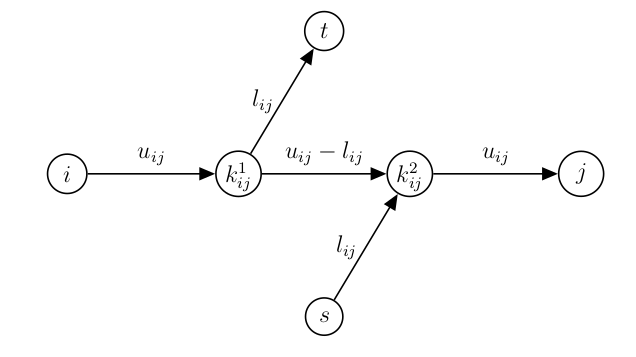
\includegraphics[width=260px]{img/edge_feasible}
    \caption{Den del af $D'$ der svarer to kanten $ij$ fra $D$ \label{edge-flow}}
  \end{figure}
  \item For at finde et feasible flow til grafen formuleres det som et maksimum flow problem, hvor man givet et flow netværk $D=(\mathcal N, \mathcal A)$ bygges et nyt flow netværk $D' = (\mathcal N', \mathcal A')$
  \begin{itemize}
  	\item Dette problem kan løses af Ford-Fulkerson eller Edmonds-Karp algoritmen
		\item $\mathcal N' = \{s,t\} \cup \mathcal N \cup \{k_{ij}^\ell \mid ij \in \mathcal A, \ell = 1,2\}$
    \item Kanterne i $D'$ der svarer til kanterne $ij \in \mathcal A$ er som beskrevet på Figur \ref{edge-flow}
    \item Fra $s$ har vi kanter til hver $i \in \mathcal N$ hvor $b_i > 0$ med øvre grænse $b_i$ 
    \item Til $t$ har vi kanter til hver $i \in \mathcal N$ hvor $b_i < 0$ med øvre grænse $-b_i$ 
    \item $D$ har et feasible flow, hvis og kun hvis $D'$ har et $(s,t)$ flow $x'$, hvor alle kanter fra source $s$ er fulde 
  \end{itemize}
  \item For at finde en argumenting cycle i en graf $D=(\mathcal N, \mathcal A)$ med nedre grænser $l_{ij}$, øvre grænser $u_{ij}$ og pris $c_{ij}$ defineres et residual netværk $D_x= (\mathcal N, \mathcal A_x)$ relativ til det nuværende flow $x$
  \begin{itemize}
  	\item Kanterne af $D_x$ indikerer hvor meget man kan ændre flowet af $x$ samtidig med at man overholder feasibility
    \item Kanterne $A_x$ af $D_x$ er følgende:
    \begin{equation*}
      \mathcal A_x = \{ij \mid ij \in \mathcal A \land x_{ij} < u_{ij} \} \cup \{ji \mid \ij \in \mathcal A \land \l_{ij} < x_{ij} \}
    \end{equation*}
    \item Når $x_{ij} < u_{ij}$ gives kanten $ij \in A_x$ den øvre grænse $(u_x)_{ij} = u_{ij} - x_{ij}$ og prisen $(c_x)_{ij} = c_{ij}$
	  \item Når $l_{ij} < x_{ij}$ gives kanten $ji \in \mathcal A_x$ den øvre grænse $(u_x)_{ji} = x_{ij} - l_{ij}$ og prisen $(c_x)_{ji} = -c_{ij}$
    \item Balancen af alle knuder er sat til $0$ 
    \item Alle knuder af $D_x$ har nedre grænse $0$ 
    \item Problemet med at finde et feasible flow i $D$ relativ til $x$ er præcist problemet med at finde negative vægtet cykler i $D_x$, når man bruger prisen som vægte. 
    \begin{itemize}
    	\item Bellman Ford eller Floyd Warshall kan bruges til dette
    \end{itemize}
  \end{itemize}
  \item \textbf{Circulation Decomposition Lemma}. Lad $x$ være en ikke negativ circulation flow i et netværk $D=(\mathcal N, \mathcal A)$. Så eksister der cykler $C_1, \dots, C_k$ og  tal $\delta_1, \dots, \delta,k \geq 0$ så ledes at
  \begin{equation*}
    x = \gamma_{C_1}^{\delta_1} + \gamma_{C_2}^{\delta_2} + \dots + \gamma_{C_k}^{\delta_k}
  \end{equation*}

  \item \textbf{Lemma} Lad $D$ være et netværk med et feaasible flow $x$. Hvis $x$ ikke er en minimum kost flow, så eksister der en augumenting cykel
  \item Siden prisen bliver bedre hver iteration, garanterer dette at algoritmen stopper  
  \item Den kører i værste tilfælde eksponentiel mange gange
\end{itemize}
% \subsubsection{Find en argumenting cykel}
% \subsubsection{Correctness}

\newpage
%%% Local Variables:
%%% mode: latex
%%% TeX-master: "optimering-noter"
%%% End:

\section{Homomorphic Encryption}
\begin{itemize}
    \item A \textbf{fully homomorphic encryption scheme (FHE)}  is like a standard encryption scheme $(\Gen, \Enc, \Dec)$ with an extra algorithm $\Eval$
    \begin{itemize}
        \item $\Eval$ takes as input a vector of ciphertexts a function $f$ and outputs an encryption of the function applied to the plaintexts i.e. for $(pk, sk) \leftarrow \Gen(1^k)$ it must be the case that
        \begin{equation*}
            \Dec_{sk}(Eval(f, \Enc_{pk}(x_1), \dots, \Enc_{pk}(x_n))) = f(x_1, \dots, x_n)
        \end{equation*}
        \item A fully encryption scheme is homomorphic with respect to any function $f$ described as a circuit
        \item A \textbf{$d$-HE scheme} allows to evaluate every function which can be expressed by a circuit with depth at most $d$ 
        \item \textbf{Compactness:} The work performed by the decryption function should be independent of the function $f$
        \begin{itemize}
            \item Since otherwise one could use the decryption algorithm to compute the function after decrypting all the inputs
        \end{itemize}
        \item An encryption scheme $(\Gen, \Enc, \Dec, \Eval)$ has \textbf{circuit privacy} with respect to a function family $\mathcal{F}$ if for all $(pk, sk) \leftarrow \Gen(1^k)$, plaintext $x$ and function $f \in \mathcal F$, it holds that
        \begin{equation*}
            (sk, \Enc_{pk}(f(\overrightarrow x))) \approx_c (sk, \Eval_pk(f, \Enc_{pk}(\overrightarrow x)))
        \end{equation*}
    \end{itemize}
    \item It can be used to do secure two party computation between two parties $\A$ and $B$ for a function $f$ as follows
    \begin{enumerate}
        \item $\A$ generates $(pk, sk) \leftarrow \Gen(1^k)$ and computes $c_1 = \Enc(pk, x_1), \dots, c_n = \Enc(pk, x_n)$ and sends $pk$ and the encrypted inputs to $\B$
        \item $\B$ encrypts its inputs $d_1 = \Enc(pk, y_1), \dots, d_n = \Enc(pk , y_n)$
        \item $\B$ runs $c =\Eval(f, c_1, \dots, c_n, d_1, \dots d_n)$ and sends it to $\A$
        \item $\A$ computes $z = \Dec(sk, c)$ and outputs $z$ 
    \end{enumerate}
    The security of this protocol follows from the security of the FHE
\end{itemize}

\subsection{Pailler's Cryptosystem}%
\begin{itemize}
    \item Pailler can be seen as a variant of the RSA encryption scheme that uses modulo $N^2$ instead of $N$
    \begin{itemize}
        \item It allows to encrypt any message in $Z_n$
        \item It is build using two "mappings" from $Z_N$ into $Z_{N^2}$
        \item The first mapping $\alpha(x)$ takes care of the messages and ensures that the scheme is homomorphic:
        \begin{equation*}
            \alpha(x) = (1+ x N) \mod N^2
        \end{equation*}
        which is homomorphic since
        \begin{align*}
            \alpha(x) \cdot \alpha(y) \mod N^2 &= (1 + xN) (1+ yN) \mod N^2 \\
                                &= (1 + xN + yN + xyN^2) \mod N^2 \\
                                &= (1 + (x + y)N) \mod N^2 = \alpha(x + y \mod N)
        \end{align*}
        this mapping is not particular secure in fact it is invertible 

        \item The second mapping $\beta(r)$ takes care of the randomness and makes sure that the scheme is secure:
        \begin{equation*}
            \beta(r) = r^N \mod N^2
        \end{equation*}
        which is homomorphic since
        \begin{align*}
            \beta(x) \cdot \beta(y) \mod N^2 &= x^N \cdot y^N \mod N^2 \\
                                             &= (x \cdot y)^N \mod N^2 \\
                                             &= \beta(x \cdot y) \mod N^2
        \end{align*}
        \item The security of Pailler encryption is based on the assumption that it is hard to distinguish between uniformly random elements in $Z_{N^2}$ and the output of $\beta(r)$ on an uniformly random $r$
        \begin{itemize}
            \item This is easy if the factorization of $N$ is known
        \end{itemize}
    \end{itemize}
    \item The Pailler cryptosystem is defined as follows
    \begin{itemize}
        \item \textbf{Key Generation:} Sample primes $p,q$ of the same length and compute $N = p \cdot q$. Output $sk = \phi(N) = (p-1)(q-1)$ and $pk = N$
        \item \textbf{Encryption:} On input a message $m \in Z_n$, sample a random $r \in Z_n^*$ and output
        \begin{equation*}
            C = \alpha(m) \cdot \beta(r) = (1 + m N) r^N \mod N^2
        \end{equation*}
    \item \textbf{Decryption:} Compute $m = \alpha^{-1}(C^{sk} \mod N^2) \cdot sk^{-1} \mod N$
    \end{itemize}
    \item The security follows from the assumption that $\beta(r)$ is indistinguishable from a random element of $Z_{N^2}$

\end{itemize}

\subsection{Bootstrapping}%
\begin{itemize}
    \item The central idea for constructing FHE is Bootstrapping:
    \begin{itemize}
        \item We are given a $d$-HE scheme $(gen, enc, dec, eval)$ where $eval$ can evaluate any circuit with depth at most $d$
        \item It is assumed that the decryption function $dec$ can be described by a "shallow" circuit with depth $d' < d$ 
        \item Using this it is possible to construct a FHE scheme that permits to evaluate circuits of any polynomial deptch
    \end{itemize}
    \item The \textbf{level} of the ciphertext is defined as 
    \begin{itemize}
        \item $0$ if it is the output of the enc function
        \item A ciphertext obtained using $c' = eval_{pk}(f,c)$ has level $i+j$ where $i$ is the level of $c$ and $j$ is the depth of the circuit $f$
    \end{itemize}
    \item An FHE scheme $(\Gen, \Enc, \Dec, \Eval)$ can be constructed as follows:
    \begin{itemize}
        \item $\Gen$ runs $(pk, sk) \leftarrow gen(1^k)$ and defines $SK = sk$ and $PK = (pk, enc_pk(sk))$
        \begin{itemize}
            \item Thus we require that the scheme is secure even when the adversary is given an encryption of the secret key
            \item It is known as a \textbf{circular secure encryption scheme} 
        \end{itemize}
        \item The encryption and decryption functions $\Enc, \Dec$ work exactly in the same way
        \item The key idea to construct $\Eval$ is the technique known as refreshing:
        \begin{itemize}
            \item Take a ciphertext $C$ at level $i$ and assume that $i \leq d$ thus it can be correctly decrypted as $m = dec_{sk}(C)$
            \item Let $f(x) = dec_x(C)$ be the circuit that decrypts ciphertext $C$ using the input $x$, using the encryption of $sk$ we can compute
            \begin{equation*}
                C' = eval(f, enc(sk))
            \end{equation*}
            this then gives us a ciphertext of $m$ of depth $d'$ which might be smaller than $i$ since this does not depend on the original level $i$
            \item To encrypt e.g. the function $\neg(ab)$ where the input is two ciphertexts $C_1$ and $C_2$ one creates the following circuit:
            \begin{equation*}
                f(x) = \neg(dec_x(C_1) \cdot dec_x(C_2))
            \end{equation*}
            on the encryption of the secret key using $eval$ giving us a ciphertext with depth $d' + 1 \leq d$ and thus decryption is still correct
            \item Any boolean circuit gate can be evaluated by repeating this process as long as necessary

        \end{itemize}
    \end{itemize}
\end{itemize}

\subsection{Example of bounded homomorphic encryption scheme}%
\begin{itemize}
    \item The following is an example of a simple $d$-HE scheme
    \begin{itemize}
        \item \textbf{Key Generation:}
        \begin{itemize}
            \item choose a big seret odd integer $p$
            \item choose big random integers $q_1, \dots, q_n$ and small integers $r_1, \dots, r_n$
            \item The secret key is $p$
            \item The public key is $y_1, \dots, y_n)$ where $y_i = p \cdot q_i + 2r_i$
        \end{itemize}
        \item \textbf{Encryption:} To encrypt a bit $m$, choose at random a subset $S$ of $\{1, \dots n\}$ and compute (over the integer)
        \begin{equation*}
            c = m + \sum_{i \in S} y_i
        \end{equation*}
        \item \textbf{Decrypt:} To decrypt compute
        \begin{equation*}
            m = ((c \mod p) \mod 2)
        \end{equation*}
    \end{itemize}
    \item Decryption works:
    \begin{equation*}
        c \mod p = m + 2 \left(\sum_{i \in S} r_i \right) + P \left(\sum_{i \in S} q_i \right) \mod p = m + 2 \left(\sum_{i \in S} r_i \right) \mod p
    \end{equation*}
    if $r_i$ are smaller enough compared to $p$, and $|S|$ is of the right side i.e. $2 \cdot \sum_{i \in S}(r_i)$ does not reduce modulo $p$ then the following must be the case
    \begin{equation*}
        (m + 2 \left(\sum_{i \in S} r_i \right) \mod p) \mod 2 = m
    \end{equation*}
    and thus decryption works
    \item The security of the protocol is related to the assumption that it is hard to recover $p$ from the public key
    \begin{itemize}
        \item without the error terms $r_i$ it would be trivial to compute $p$
        \item it is believed that adding the noise it becomes hard to compute $p$ (known as the \textbf{approximate GCD problem} )
    \end{itemize}
    \item The scheme is homomorphic since if $c_1 = enc(m_1, S_1)$ and $c_2 = enc(m_2, S_2)$
    \begin{equation*}
        c_1 + c_2 \mod p = (m_1 + m_2) + 2\left(\sum_{i \in S_1}r_1\right) + 2\left(\sum_{i \in S_2}r_i \right)
    \end{equation*}
    and that 
    \begin{equation*}
        c_1 \cdot c_2 \mod p = (m_1 \cdot m_2) + 2 \left(m_1 \cdot \sum_{i\in S_2}r_i + m_2 \cdot \sum_{i\in S_2}r_i + \sum_{i\in S_1, j\in S_2}r_ir_j \right)
    \end{equation*}
    every homomorphic operation make the noise grow significantly and thus they must have some bound on the depth of function they can compute


\end{itemize}

\section{Symmetric (secret-key) Authentication and Hash Functions}
\begin{itemize}
  \item The authentication systems are used to make sure that the received message is what the sender intended
  \begin{itemize}
  	\item The Adversary can only change the message
  	\item Adversary can both change the message and authenticator
  \end{itemize}
\end{itemize}

\subsection{Hash Functions}
\begin{itemize}
  \item A hash function is defined by a \textbf{generator} $\mathcal H$, which on input a security parameter $k$ outputs the description of a function $h : \{0,1\}^* \to \{0,1\}^k$
  \item \textbf{Definition 10.1} The game where one runs $\mathcal H$ on input $k$ to get function $h$. If $A$ is given to adversary algorithm $A$ who outputs 2 strings $m,m'$ $A$ has success if $m \neq m'$ and $h(m) = h(m')$ $\mathcal H$ is collision intractable if any polynomial time $A$ has success with negligible probability as a function of $k$
  \item Collision-intractable hash functions exist under well-known intractability assumptions
  \item $\mathcal H$ is defined as follows:
  \begin{itemize}
  	\item Choose a prime $\alpha$, $\beta$ of order $q$ in $\mathbb Z_p^*$
  	\item Define a function $h : Z_q \times Z_q \to Z_p$ as follows $h(m_1, m_2) = \alpha^{m_1} \beta^{m_2} \text{ mod } p$
  	\item This is a discrete log hard problem in $\mathbb Z_p^*$ and this family of functions is collision intractable
  \end{itemize}
  \item \textbf{Lemma 10.2} Given function $h : \{0,1\}^{k+1} \to \{0,1\}^k$, and assume a algorithm $A$ are given running in time $t$ that, when given $h(m)$ for uniform $m$. return a preimage of $h(m)$ with probability $\epsilon$. Then a collision for $h$ can be found in time $t$ plus one evaluation of $h$ and with probability at least $\epsilon/4$
  \item \textbf{Theorem 10.3} If there exists a collision-intractable has function generator $\mathcal H'$ producing functions with finite input length $m >k$, then there exists a collision-intractable generator $\mathcal H$ that produces functions taking arbitrary length input. \smallskip \\
  \textbf{Proof} \\
  The case where $m-k > 1$ 
  \begin{itemize}
    \item Set $v = m-k-1$ and note that $v> 0$ 
    \item Now the generator $\mathcal H$ is defined
    \item $H'$ is used to get function $f: \{0,1\}^m \mapsto \{0,1\}^k$ 
    \item The new function $h: \{0,1\}^* \mapsto \{0,1\}^k$ as follows 
    \begin{itemize}
    	\item Split the input string $x$ in $v$ bit blocks $x_1, \dots, x_n$ padding the last block with $0$s if needed
      \item Add a block $x_{n+1}$ containing in binary notation the number of $0$s used in padding $x_n$
      \item Define a series of $m$ bit blocks $z_1, z_2, \dots, z_{n+1}$ as follows set 
      \[
        z_1 = 0^k \mid \mid 1 \mid \mid x_1
      \]
      and for $i=2,\dots,n+1$ set
      \[
        z_i = f(z_{i-1}) \mid \mid 0 \mid \mid x_i
      \]
      define $h(x) = f(z_{n+1})$
      \item The single bit fields in the middle is used for distinguishing the starting state from all intermediate states
    \end{itemize}
    \item $h$ is shown to be collision intractable by contradiction i.e. if one can find a collision for $h$ one can efficiently find one for $f$
    \begin{itemize}
      \item Assume that we are given $x \neq x'$ where $h(x) = h(x')$
      \item Let $z_1, \dots, z_{n+1}$ and $z_1',\dots, z_{n'+1}'$ be the sequence of inputs to $f$ as defined when processing $x$ and $x'$ in $h$ 
      \item Assume without loss of generality that $n \geq n'$ 
      \item By assumption it is known that $f(z_{n+1}) = h(x) = h(x') = f(z_{n+1}')$
      \item There are two cases either
      \begin{itemize}
      	\item $z_{n+1} \neq z'_{n'+1}$ which gives a collision for $f$ 
        \item Or $z_{n+1} = z'_{n'+1}$ which implies that the number of $0$'s used for padding $x_n$ and $x'_{n'}$ are equal and $f(x_{n-1}) = f(x'_{n' -1 })$ 
      \end{itemize}
      This argument can be repeated and this claim must lead to a collision for $f$
      \item If this did not lead to a collision then the inputs to $f$ are equal and one would eventually reach a stage where one could conclude $z_{n-n'+1} = z'_1$ at this point one would also have
      \[
        x_{n+1} = x'_{n'+1}, x_{n} = x'_{n'}, \dots, x_{n-n'+1} = x_1'
      \]
      this cannot if $n = n'$ since this would imply $x = x'$ which would be false by assumption and if $n > n'$ then it cannot be the case that $z_{n-n'+1} = z_1 '$ because then $z_{n-n' +1}$ has a $0$ in position $k+1$ while $z_1'$ has a $1$
    \end{itemize}
  \end{itemize}
  The case where $m-k = 1$ 
  \begin{itemize}
  	\item A function $\overline{h}$ is constructed from $f$ 
    \begin{itemize}
      \item Define $z_1 = 0^k \mid \mid x_1$ where $x_1$ is the first bit of $x$
      \item Then for $i = 2,\dots,n+1$ set
      \[
        z_1 = f(z_{i-1}) \mid \mid x_i
      \]
      \item Define $\overline{h}(x) = f(z_{n+1})$
    \end{itemize}
    \item The function $\overline{h}$ will be modified to get the actual hash function $h$ 
    \item The only time $\overline{h}$ produces a collision where $f$ does not produce a collision is when $x'$ is a suffix of $x$ where $n > n'$ 
    \item Define $h(x) = \overline{h}(E(x))$ where $E()$ is a suffix-free encoding 
    \begin{itemize}
    	\item A suffix-free encoding is an with the property that there exist no pair $x,xø$ such that $E(x')$ is a suffix of $E(x)$
      \item It is clear that a collision for $h$ implies a collision for $f$ 
    \end{itemize}
    \item A suffix-free encoding can be constructed by defining $D()$ as the function which repeats every bit twice
    \[
      D(x_1, \dots, x_n) = x_1x_1 \dots x_nx_n
    \]
    let $E(x) = 01 \mid \mid D(x)$
  \end{itemize}
  \item \textbf{Theorem 10.4} Given function $h$, and assume that it is possible to sample input values to $h$ causing the outputs to be uniformly random in $\{0,1\}^k$. Then a collision for $h$ can be found with constant probability in time corresponding to $2^{k/2}$
\end{itemize}

\subsubsection{The random oracle model}
\begin{itemize}
  \item In the Random Oracle Model the idea is formalized that the output values "might as well" be random
  \begin{itemize}
  	\item The idea is that the hash function is replaced with a random oracle
  	\item A \textbf{random oracle} is a oracle that will receive any string $m$ as input and will return a randomly chosen $R(m)$
    \begin{itemize}
  		\item If it later receives the $m$ as input, the same string $R(m)$ will be returned
    \end{itemize}
  	\item Every time a new string $m'$ is given as input a fresh random string $R(m')$ is returned chosen independently
  	\item Every including the adversary has acces to such an oracle and it is the same oracle for everyone
  \end{itemize}
  \item In the real life one does not have access to some random oracle but one can hope that the adversary can only do as good as in the random oracle case
  \item If an application of an hash function has been proven secure in the random oracle model, this means that for the real life application is that any attack that considers the has function $h$ as a "random black-box" and does not use any special properties of $h$ is doomed to failure
\end{itemize}

\subsection{MACs}
\subsubsection{Definition}
\begin{itemize}
  \item A \textbf{secret-key authentication system} consists of three probabilistic algorithms $(G,A,V)$
  \begin{itemize}
  	\item $G$ which outputs a key $K$
    \begin{itemize}
  		\item One usually works by simply choosing $K$ as a random bit string of a certain length
    \end{itemize}
  	\item $A$ gets input a message $m$ and the key $K$ and outputs an authenticator value $s = A_K(m)$
  	\item $V$ gets as input an input $s$, a message $m$ and key $K$ and outputs $V_K(s,m)$ which is equal to \textit{accept} or \textit{reject} 
    \begin{itemize}
  		\item It is required that the following always hold $V_K(A_K(m),m) = accept$
    \end{itemize}
  \end{itemize}

  \item A secret-key authentication system is called a MAC scheme
  \begin{itemize}
  	\item MAC stands for message authentication codes (MACs)
  	\item MAC is also the name for the authenticator value $s$
  \end{itemize}
\end{itemize}

\subsubsection{Security}
\begin{itemize}
  \item \textbf{Definition 10.5 (CMA Security of MACs)} A MAC scheme is $(t,q,\epsilon, \mu)$ CMA-secure if any adversary that runs in time at most $t$ and asks at most $q$ queries, on messages of total length $\mu$ bits, wins the following game with probability at most $\epsilon$
  \begin{itemize}
  	\item Given some system $(G,A,V)$, the adversary $E$ gets access to an oracle
    \begin{itemize}
  		\item Which initially runs $G$ to get $K$
    \end{itemize}
  	\item $E$ may as many times as it wants send some message $m$ to the oracle who will return to $E$ the MAC $A_K(m)$
    \begin{itemize}
  		\item i.e. $E$ gets to do a chosen message attack (CMA)
    \end{itemize}
  	\item At the end of the game, $E$ outputs a message $m_0$ and an authenticator $s_0$
  	\item $E$ wins the game if $m_0$ is not one of the message the oracle was asked to authenticate and $V_K(a_0,m_0) = accept$
  \end{itemize}
\end{itemize}

\subsection{MACs from block ciphers}
\begin{itemize}
  \item The most well-known scheme for MAC's is called CBC-MAC and is based on block ciphers
  \begin{itemize}
  	\item Given a block cipher system one encrypts the input mesage in CBC mode using $IV = 0$ and define the MAC to be the final block of the ciphertext
  	\item Therefore the MAC has fixed length no matter how long the message is
  \end{itemize}

  \item EMAC is the following scheme which solves the problem of blocks having to be divisible by $k$
  \begin{itemize}
  	\item Define a new MAC scheme using 2 keys $K_1$, $K_2$
  	\item Compute the CBC-MAC on the message using $K_1$
  	\item This MAC is encrypted under $K_2$ and the output is the result of this
  	\item It is formally defined as
  \end{itemize}
  \begin{equation}
    E M A C_{K_{1}, K_{2}}(m)=E_{K_{2}}\left(C B C-M A C_{K_{1}}(m)\right)
  \end{equation}

  \item \textbf{Theorem 10.6} Suppose the block cipher $(G,E,D)$ is a $(t',q',\epsilon')$ secure PRF and has block length $k$. Then EMAC based on this block-cipher is a $(t,q,\epsilon, \mu)$ CMA-secure MAC scheme, where
  \begin{equation}
    t \leq t^{\prime}, \quad \mu / k \leq q^{\prime}, \quad \epsilon=2 \epsilon^{\prime}+\frac{2(\mu / k)^{2}+1}{2^{k}}
  \end{equation}
\end{itemize}

\subsection{MACs from hash functions}
\begin{itemize}
  \item HMAC is a MAC scheme based on any collision intractable hash function

  \item The following is a HMAC based on SHA-1
  \begin{itemize}
  	\item The key is a random 512-bit string $K$
  	\item The scheme uses two 512 bit constant $ipad = 3636 \dots 36$, $opad = 5C5C \dots 5C$ in HEX notation
  	\item The function is defined as follows:
    \begin{equation}
      HMAC_{K}(m)=S H A 1((K \oplus opad)\|S H A 1((K \oplus ipad) \| m))
    \end{equation}
  \end{itemize}
  It can be proved secure in the random oracle model
  \item HMAC is secure if the hash function is collision resistant and if the and if the basic compression function is secure in a weak sense when used as MAC

\end{itemize}

\newpage

%%% Local Variables:
%%% mode: latex
%%% TeX-master: "crypto-noter"
%%% End:

\section{Approximation Algorithms and Local Search Heuristics.}
\begin{itemize}
	\item \textbf{Kompleksitetsklassen} $\mathbf P$ er klassen af sprog, der kan blive besluttet i polynomiel tid af en Turing maskine
	\item \textbf{NP} er klassen af sprog $L$ hvor der eksister et sprog $L' \in \mathbf P$ og et polynomium $p$ således at
  \begin{equation*}
    \forall v: x \in L \Leftrightarrow [\exists y \in \{0,1\}^* : |y| \leq p(|x|) \land \langle x, y \rangle \in L']
  \end{equation*}
  \item Given to sprog $L_1$ og $L_2$ reducerer $L_1$ til $L_2$, hvis der er en polynomiel udregnelig funktion $r$ således at for alle $x \in \{0,1\}^*$ har at
  \begin{equation*}
    x \in L_1 \Leftrightarrow x \in L_2
  \end{equation*}
  Skrevet som $L_1 \leq L_2$ 
  \item Et sprog $L$ er et $\mathbf{NP}$ hård sprog, hvis den har den egenskab af for alle $L' \in \mathbf{NP}$, $L'$ reducerer til $L$ 
  \item Klassen $\mathbf{NPC}$ er klassen af $\mathbf{NP}$ komplette sprog, som er de sprog i $\mathbf{NP}$ som er $\mathbf{NP}$ hårde.
\end{itemize}

\subsection{Approximation algoritmer}
\begin{itemize}
	\item En approximations algoritme er en algoritme, der prøver at approximere et NP komplet problem i polynomiel tid.
  \item En algoritme for et problem har en \textbf{approximationsratio} på $p(n)$, hvis for et hvert input af størrelse $n$, pris $C$ af løsning er inden for en faktor af $p(n)$ af den optimal løsning $C^*$ 
  \begin{equation*}
    \max\bigg(\frac C{C^*} \frac{C^*}{C} \bigg) \leq p(n)
  \end{equation*}
  \item Hvis en algoritme har en approximationsratio på $p(n)$ kaldes det for en $p(n)$ approximationsalgoritme
\end{itemize}

\subsubsection{Vertex cover}
\begin{itemize}
\begin{figure}[ht]
	\centering
\begin{lstlisting}
APPROX-VERTEX-COVER(G)
  $C= \emptyset$
  $E' = G.E$
  while $E' \neq \emptyset$
    lad $(u,v)$ være en arbritær kant i $E'$ 
    $C = C \cup \{u,v\}$
    fjern fra $E'$ alle kanter til $u$ eller $v$ 
  return $C$
\end{lstlisting}
	\caption{Approximationsalgoritme til vertex cover problemet\label{fig:approx-vertex}}
\end{figure}

  \item Et \textbf{vertex cover} af en undirected graf $G=(V,E)$ er et subset $V' \subseteq V$ således at hvis $ij \in V$ så er enten $i \in V'$ eller $j \in V'$ eller begge. 
  \item \textbf{Vertex-cover} problemet er at finde et vertex cover af en minimum størrelse givet en undirected graf. Et sådan cover er kaldt et \textbf{optimal vertex cover} og problemet er et \textbf{NP} komplet problem. 
  \item \textbf{Theorem} APPROX-VERTEX-COVER (Figur \ref{fig:approx-vertex}) er en polynomiel tid 2 approximationsalgoritme for vertex cover
  \begin{proof} 
    Algoritmen kører i polynomieltid, da den kigger på være knude og hver kant en gang dvs. at den kører i $O(|V| + |E|)$ \smallskip
  
    Algoritmen finder et vertex cover siden den looper indtil alle kanter $G.E$ er blevet dækker af en af en vertex \smallskip

    For at vise at det er en 2-approximationsalgoritme lader vi $A$ være den mængde af kanter, som bliver valgt af APPROX-VERTEX-COVER. For at dække alle kanter må et optimal cover $C^*$ indeholde mindst et af punkterne fra være af kanterne. Siden ingen kanter i $A$ deler et slut punkt får vi følgende nedre grænse
    \begin{equation*}
      |C^*| \geq |A|  
    \end{equation*}
    Siden begge endepunkter af kanterne i $A$ bliver valgt får vi følgende lighed:
   \begin{equation*}
      |C| = 2|A| 
   \end{equation*}
    Ud fra disse denne lighed og ulighed får vi approximationsratio
    \begin{equation*}
      |C| = 2|A| \leq 2|C^*|
    \end{equation*}
    Dette beviser dermed theoremet

  \end{proof}
\end{itemize}

\subsubsection{The traveling-salesman problem}
\begin{figure}[ht]
    \centering
\begin{lstlisting}
APPROX-TSP-TOUR($G$,$x$)
  lad en arbritær vertex $r\in G.V$ til at være roden
  udregn et minumum spanning tree $R$ for $G$ fra roden $r$ vedhjælp af MST-PRIM($G$, $c$, $r$)
  lad $H$ være en list af kanter, der er ordnet efter hvornår de først er blevet besøg i en tree walk af $T$
  return hamiltonian cykel $H$
\end{lstlisting}
    \caption{2 Approximationsalgoritme for TSP med trekantsuligheden \label{fig:approx-tsp-tour}}
\end{figure}

\begin{itemize}
	\item Traveling-salesman problemet er man givet en komplet undirected graf $G = (V,E)$, der har en pris $c(u,v)$ associerede med alle kanter $(u,v) \in E$. Målet er at finde den Hamilton cycle af $G$ der har den mindste kost
  \begin{itemize}
    \item TSP er et NP komplet problem
    \item Lad $c(A)$ være den totale pris af kanterne i delmængden $A \subseteq E$ 
    \item En cost funktion $c$ overholder \textbf{trekantsuligheden}, hvis alle knuder $u,v,w \in V$ følgende gælder
    \begin{equation*}
      c(u,w) \leq c(u,v) + c(v,w) 
    \end{equation*}
    \item TSP problemet der overholder trekantsuligheden er også NP komplet
  \end{itemize}
  \item APPROX-TSP-TOUR (Figur \ref{fig:approx-tsp-tour}) har en kørertid på $\Theta(V^2)$ 
  \item \textbf{Theorem} APPROX-TSP-TOUR (Figur \ref{fig:approx-tsp-tour}) er en polynomiel-tids 2-approximationsalgoritme for TSP der overholde trekantsuligheden
  \begin{proof} 
    Algoritmen kører i polynomieltid siden MST-PRIM kører i $\Theta(V^2)$ \smallskip
    
    Lad $H^*$ være den optimal tour for et given set af knuder. Vi får et spanning tree ved at slette en hvilken som helst kant. Dette medfører at det MST $T$ der bliver udregnet må være en nedre grænse for $H^*$:
    \begin{equation*}
      c(T) \leq c(H^*) 
    \end{equation*}
    Lad $W$ være en \textbf{full walk} af træet $T$, der lister hvornår en given knude er besøgt og hvornår man kommer tilbage til denne knude efter at have besøgt et subtræ. Siden man bruger hver kant to gange får man følgende lighed
    \begin{equation*}
      c(W) = 2c(T) 
    \end{equation*}
    Siden $W$ besøger nogle kanter to gange er det ikke en hamiltonian path. Dog ved vi per trekantsuligheden at vis man går hen til knuderne direkte får man en bedre rute derfor må der gælde at:
    \begin{equation*}
      c(H) \leq c(W)
    \end{equation*}
    Hvis bruger disse får man følgende
    \begin{equation}
      c(H) \leq c(W) = 2c(T) \leq 2c(H^*) 
    \end{equation}
    Dermed er det bevist at algoritmen har en approximationsratio på 2.

  \end{proof}
  \item \textbf{Theorem} Hvis $\mathbf{P} \neq \mathbf{NP}$, så for enhver konstant $\rho \geq 1$, er der ingen polynomiel tids approximationsalgoritme med approximationsratio $\rho$ for den generelle TSP 
  \begin{proof} 
    Antag for modstrid, at der eksistere en approximationsalgoritme $A$ med en approximationsratio på $\rho$ og at $\mathbf{P} \neq \mathbf{NP}$. Det vises at vis dette er tilfældet kan Hamilton cycle problem blive løst i polynomiel tid. \smallskip

    Lad $G=(V,E)$ være et Hamilton problem. Vi definerer det tilsvarende TSP problem $G'=(V, E')$, hvor 
    \begin{equation*}
      E' = \{(u,v) \mid u,v \in V, u \neq v \}
    \end{equation*}
    Pris funktionen defineres på følgende måde
    \begin{equation*}
    	c(u,v) =
    		\begin{cases}
    			\mbox{$1$} & \mbox{hvis $(u,v) \in E$} \\
    			\mbox{$\rho|V| + 1$} & \mbox{ellers} \\
    		\end{cases}
    \end{equation*}    
    Dette kan blive konstrueret i polynomiel tid i $|V|$ og $|E|$. \smallskip
    
    Hvis den originale graf havde en Hamilton cycle, så må den optimale path have værdi $|V|$. Derfor må den kun vælge kanter af den Hamilton cycle siden, hvis den bruger en kant $(u,v) \notin E$ har den en kost på mindst 
    \begin{equation*}
      (\rho |V| +1) + (|V| -1) = \rho |V| + |V| > \rho |V| 
    \end{equation*}
    Siden at tage denne kant med medfører, at den samlede pris bliver mere end $\rho$ gange så meget som den optimale løsning vil vores approximationsalgoritme ikke vælge den hvis der eksisterer en Hamilton path. \smallskip

    Dermed kan man bruge en sådan algoritme $A$ til at finde Hamilton path. Siden man bare skal tjekke hvorvidt den resulterende path har en kost $C > \rho |V|$. Derfor kan man afgøre det i polynomiel tid og det kan ikke lade sig gøre hvis $\mathbf{P} \neq \mathbf{NP}$ og dette medfører at vi får en modstrid. 

  \end{proof}
\end{itemize}

\subsubsection{Randomisering}
\begin{itemize}
	\item En randomiseret algoritme for et problem har n approximationsratio $p(n)$, hvis for ethvert input af størrelse $n$ er den forventede pris $C$ af en løsning produceret af algoritmen er inden for en factor $p(n)$ af prisen $C^*$ af den optimale løsning:
  \begin{equation*}
    \max\bigg(\frac{C}{C^*},\frac{C^*}{C}\bigg) \leq p(n)
  \end{equation*}
  \item En \textbf{randomiseret} $p(n)$ \textbf{approximationsalgoritme} er en randomiseret algoritme der har en approximationsratio ratio på $p(n)$ 
  \item \textbf{MAX3CNF SAT} er problemet af at finde en assigment der maksimere antallet af satisfied clauses 
  \item \textbf{Theorem} Givet en tilfælde af MAX3CNF SAT med $n$ variabler $x_1, x_2, \dots, x_n$ og $m$ clauses, er den randomiseret algoritme der sætter hver variable til at være $1$ med sandsynlighed en $1/2$ og $0$ med sandsynlighed $1/2$ er en randomiseret $8/7$ approximationsalgoritme.
  \begin{proof} 
    Lad os antage, at vi har sat variabler uafhængig til $1$ med sandsynlighed $1/2$ og $0$ med sandsynlighed $1/2$. Så for $i=1,\dots,m$ defineres den random variable 
  \begin{equation*}
    Y_i = I\{\text{clause $i$ er satisfied}\}
  \end{equation*}  
  Det vil sige at clause $I$ er satisfied, så længe en af dens literals er sat til $1$. Siden at vi har antaget at hver literal kun forekommer engang og at en variable og dens negation ikke forekommer sammen er de tre literals i hver clause uafhængige. \smallskip

  Dermed får vi følgende forventede værdi af en given clause
  \begin{align*}
    E[Y_i] = \text{Pr}\{\text{clause $i$ er satisfied}\} &= 1- \text{Pr}\{\text{clause $i$ er ikke satisfied}\} \\
                                                         &= 1- \bigg(\frac12 \bigg)^3 = \frac78
  \end{align*}
  Lad $Y$ være det samlede antal af satisfied clauses, således at $Y = Y_1 + Y_2 + \cdots + Y_m$ så har vi at
  \begin{align*}
    E[Y] &= E\bigg [ \sum_{i=1}^m Y_ i\bigg] \\
         &= \sum_{i=1}^m E[Y_i] \\
         &= \sum_{i=1}^m \frac78 \\
         & = \frac{7m}8
  \end{align*}
  Siden $m$ er den øvre græse for hvor mange satisfied clauses, der kan være får vi en approximationsratio på $m/(7m/8)=8/7$  

  \end{proof}
\end{itemize}

\subsubsection{Lineær programmering}
\begin{figure}[ht]
  \centering
\begin{lstlisting}
APPROX-MIN-WEIGHT-VC($G$, $w$)
  $C = \empty$ 
  udregn $\bar x$ som er en optimal løsning til det lineær program relaxation
  for hver $v \in V$ 
    if $\bar x(x) \geq 1/2$
      $C = C \cup \{v\}$
  return $C$
\end{lstlisting}
  \caption{Approximationsalgoritme for minimum vægt vertex-cover problemet\label{fig:vertex-min-weight}}
\end{figure}

\begin{itemize}
	\item I \textbf{minimum vægt vertex-cover problemet} er man givet en undirected graf $G=(V,E)$ hvor hver vetex har en positiv vægt $w(x)$. For ethvert vertex cover $V' \subset V$ defineres vægt af vertex coveret til at være $w(V') = \sum_{v \in V'} w(v)$. Målet er af finde vertex coveret med minimm vægt
  \item Minimum vægt vertex-cover problemet kan blive formuleres som følgende integer lineær program hvor $x(v)$ definere hvorhvidt $v$ er med i vertex coveret eller ej
  \begin{alignat*}{2}
    \text{min} \quad  & \sum_{v \in V} w(v) x(x) && \\
    \text{s.t.} \quad & x(u) + x(v) \geq 1 && \quad \text{for hver } (u,v) \in E \\
    & x(v) \in {0,1} && \quad \text{for hver } v \in V
  \end{alignat*}
  \item Hvis restrektionen af $x(v) \in \{0,1\}$ er fjernet fået følgende \textbf{lineær programmerings relaxation} fåes
  \begin{alignat*}{2}
    \text{min} \quad  & \sum_{v \in V} w(v) x(x) && \\
    \text{s.t.} \quad & x(u) + x(v) \geq 1 && \quad \text{for hver } (u,v) \in E \\
    & x(v) \leq 1 && \quad \text{for hver } v \in V \\
    & x(v) \geq 0 && \quad \text{for hver } v \in V
  \end{alignat*}
  Dette giver en nedre grænse på værdi af den optimale løsning til 0-1 integer programmet
  \item \textbf{Theorem} Algoritmen APPROX-MIN-WEIGHT-VC (Figur \ref{fig:vertex-min-weight}) er en polynomiels tid 2-approximationsalgoritme for minimum vægte vertex cover problemet
\end{itemize}

\subsubsection{Approximations schemes}
\begin{itemize}
	\item Et \textbf{approximation scheme} for et optimeringsproblem er en approximationsalgoritme der ud over problemet også tager et $\epsilon >0$ således at for en fast $\epsilon$ er schemet et $(1+\epsilon)$ approximationsalgoritme. 
  \begin{itemize}
		\item Det er en \textbf{polynomiel tid approximationsscheme} hvis for et fixed $\epsilon >0$ kører schemet i polynomiel tid i størrelsen $n$ af den input instance
    \item Det er en \textbf{fully polynomiels tid approximationsscheme} hvis den er en approximations scheme og den kører i polynomiel i både $1/ \epsilon$ og størrelse $n$ af input instancen.
  \end{itemize}
  \begin{figure}[ht]
    \centering
\begin{lstlisting} 
  $V \leftarrow \max\{v_i \mid w_i \leq W\}$
  $B \leftarrow \epsilon V /n$
  $v_i' \leftarrow \lfloor v_i / B \rfloor$
  Udregn den optimale løsning $S'$ ved hjælp af vægte $w_1, \dots w_2$ nye værdier $v_1', \dots, v_n'$ og vægt limit $W$ vha. en dynamisk programmeringsalgoritme
  return $S'$ 
\end{lstlisting}
    \caption{ $\epsilon$-approximation algorithm for Knapsack\label{fig:approx-knapsack}}
  \end{figure}

  \item \textbf{Knapsack problemet} er følgende problem: Givet vægte $w_1, \dots w_n$, værdier $v_1, \dots, v_n$ og en vægt limit $W$ find $S \subseteq \{1,\dots,n\}$ der maksimere $\sum_{i \in \mathcal S} v_i$ og overholder $\sum_{i \in S} w_i \leq W$ 
  \item \textbf{Theorem} Algoritmen på Figur \ref{fig:approx-knapsack} kører i $O(n^3 / \epsilon)$ tid og har en approximationsratio på $(1- \epsilon)$
\end{itemize}


\subsection{Local search heuristikker}
\begin{itemize}
	\item Local search er en type af approximationsalgoritmer der givet en løsning prøver at finde en bedre løsning ved hjælp af en form for ændring på den nuværende løsning
\end{itemize}
\subsubsection{Tur konstruktions heuristikker}
\begin{itemize}
	\item For at finde en bedre TSP tour bliver der brugt en heuristik.
  \item En heuristik kan bliver evalueret på to punkter: dens køretid og kvaliteten af den tour den producerer
  \item En heuristik er undominated hvis der ikke eksister en anden heuristik der både finde en bedre tour og køre hurtigere
  \item \textbf{Nearest Neighbour} 
  \begin{itemize}
  	\item vælger den by som er tættest på
    \item starter med at vælge en arbritær by 
    \item køretiden er $\Theta(N^2)$
    \item approximationsratio er $(0.5)(\log_2N + 1)$
  \end{itemize}
  \item \textbf{Greedy}
  \begin{itemize}
  	\item En tour bliver bygget ved at vælge den mindste kant i grafen indtil der er en TSP
  	\item køretiden er $\Theta(N^2 \log N)$
  	\item approximationsratio er $(0.5)(\log_2N + 1)$
  \end{itemize}
  \item \textbf{Clarke-Wright}
  \begin{itemize}
  	\item starter med en tour hvor alle går igennem en arbritær valgt ``hub'' by
    \item fjerner en kant og vælger den nye kant der sparer flest penge
    \item stopper når der kun er 2 non hub byer tilbage
    \item køretiden er $\Theta(N^2 \log N)$ 
    \item Den har en approximationsratio på $\log N +1$ 
  \end{itemize}
  \item \textbf{Christofides}
  \begin{itemize}
  	\item Den prøver at finde en bedre Euler tour $W$ på følgende måde:
    \begin{itemize}
    	\item Udregn MST $T$
      \item Lad $V_{\text{odd}}$ være byer med en ulige degree i $T$
      \item Udregn min cost perfect matching $M$ på $V_\text{odd}$
      \item Find Euler tour $W$ fra $T \cup M$
      \item Tag genveje for at få $H$
    \end{itemize}
    \item Den har en approximationsratio $3/2$
  \end{itemize}
\end{itemize}

\subsubsection{Natural neighborhood for TSP}
\begin{itemize}
	\item $k$ OPT for $k = 2, 3, 4, \dots$ 
  \begin{itemize}
  	\item Fjern $k$ kanter fra en tour, og tilføj $k$ kanter til at finde en anden tour 
    \item De kan gøres hurtigere med følgende:
    \begin{itemize}
    	\item Neighbour lists
    	\item Prune lists til 20 elementer
    	\item Don't look bits
    \end{itemize}
    \item 3-OPT er feasible endda for millioner af byer
  \end{itemize}
  \item For at gøre local search bedre kan man bruge meta heuristikker til sørger for man kan komme ud af lokale optimums
  \item \textbf{Taboo search} 
  \begin{itemize}
    \item Den generelle strategi er at finde en lokalt optimum og når et er blevet fundet at identificere den bedste løsning tæt på som kan blive brugt til en ny local optimeringsfase
    \item De valg der er blevet brugt til at finde den bedste løsning ligger i en \textbf{tabu list}  som bliver brugt til at diskvalificere ny valg der vil modvirker tidligere valg
  \end{itemize}
  \item \textbf{Lin-Kernighan Search} 
  \begin{figure}[ht]
    \centering
    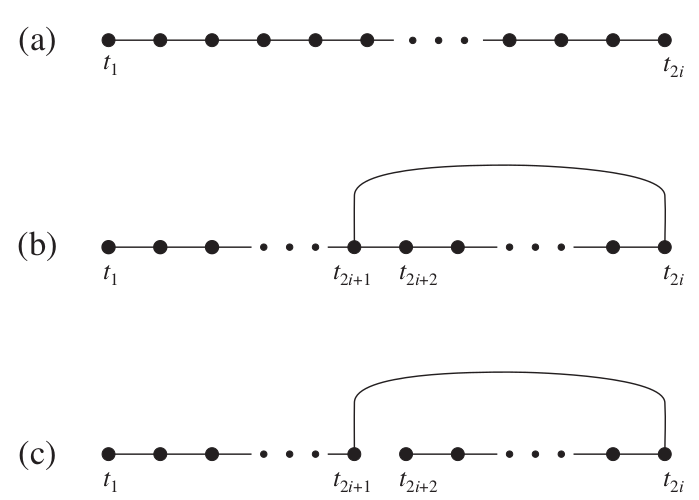
\includegraphics[width=300px]{img/lin_kernighan_move}
    \caption{A Lin-Kernighan move\label{fig:kernig}}
  \end{figure}
  \begin{itemize}
    \item Den er baseret til at subset af 2-opt valg
    \item \textbf{Ancor} af den nuværende path er en fixed slut by $t_1$
    \item Lad $t_{2i}$ være den anden ende af path $P_i$, der eksistere i step $i$ af LK search
    \item Den nuværende tour for den nuværende path $P_i$ fåes ved at tilføje kanter $t_{2i}, t_1$ 
    \item Kun 2 OPT valg som flipper et suffix af pathen altså valget hvor en af tour kanterner der bliver fjernet er $\{t_1, t_{2i}\}$ se Figur \ref{fig:kernig}
    \item Den nye nabo $t_{2i+1}$ af $t_{2i}$ må være længde af spanning træet plus en kant mindre end længden af den bedste tur ind til videre
    \item Den kan med fordel bruges flere gange for at få et bedre resultat
  \end{itemize}
  \item \textbf{Simulated anealing} 
\begin{figure}[ht]
  \centering
\begin{lstlisting}  
Generer en start løsning $S$
Sæt den initiellle bedste løsning $S^* = S$ 
Find ud af en start temperatur $T$
while not fronzen gør følgende 
  while not at equilibrium
    Vælg en random neighbour $S'$
    Sæt $\Delta = Length(S') - Length(S)$
    if $\Delta \leq 0$
      Sæt $S=S'$
      if $Length(S) < Length (S^* )$ sæt $S^* = S$  
    else 
      Vælg et random tal $r$ uniformt i $[0,1]$
      Hvis $r < e^{-\Delta/T}$ sæt $S=S'$
  Gør temperaturen $R$ lavere
return $S^* $
\end{lstlisting}
  \caption{Simulated anealing algoritme\label{fig:simulated-anealing}}
\end{figure}
  \begin{itemize}
  	\item Algoritmen kan ses på Figur \ref{fig:simulated-anealing}
    \item Hvis man gør temperaturen lavere i en rate af $C/\log n$ hvor $n$ er antallet af steps finder den optimale værdi, det er dog meget langsommere end exhaustive search 
    \item Temperaturen bliver typisk gjort lavere meget hurtigere, hvilket giver en approximationsalgoritme
  \end{itemize}
  \item \textbf{Evolutionary algortime} 
\begin{figure}[ht]
  \centering
\begin{lstlisting}  
Generere en population af $k$ start løsninger $S=\{S_1, \dots, S_k\}$
Brug en lokal optimeringsalgoritme $A$ til at løsningerne $S$ i $S$
lad den resulterende løsning erstatte $S$ 
while not converged
  Vælg $k'$ distincte subsets af $S$ af størrelse 1 eller 2 som Forældre
  for hver 1 elements subset udfør en tilfældig mutation for at få en ny løsning 
  for hver 2 elements subset udfør en crossover operation for at få en ny løsning 
  Brug $A$ på hver af de $k'$ løsninger produceret
  lad $S'$ være de resulterende løsninger
  En selection strategi bliver brugt til at vælge $k$ løsninger fra $S \cup S'$
return best solution fra $S$  
\end{lstlisting}
  \caption{Genetisk optimeringsalgoritme\label{fig:evolutionary}}
\end{figure}
  \begin{itemize}
  	\item En generel evolutionel algoritme er beskrevet på Figur \ref{fig:evolutionary}
  \end{itemize}
\end{itemize}

\newpage
%%% Local Variables:
%%% mode: latex
%%% TeX-master: "optimering-noter"
%%% End:

\section{Basic Separation Logic: Specs and Proof for Abstract Data Types}
\subsection{Basic Seperation Logic}
\subsubsection{Star magic wand and weak rule}
\begin{itemize}
  \item A proposition $P$ escribes a set of resources
  \begin{itemize}
  	\item $\mathcal R$ is used for the set of resources and $r_1$, $r_2$ etc. for elements in $\mathcal R$
    \item It is assumed that 
    \begin{itemize}
    	\item There is an empty resource
      \item There is a way to compose resources $r_1$ and $r_2$ denoted $r_1 \cdot r_2$
      \item The composition defindes for resources are disjoint denoted $r_1 \# r_2$
    \end{itemize}
  \item The intuition for $P \vdash Q$ is that all resources in $P$ are also in $Q$ i.e.
  \begin{equation*}
    \forall r \in \mathcal R. r \in P \Rightarrow r \in Q 
  \end{equation*}
  \end{itemize}
  \item $P*Q = \{r \mid \exists r_1, r_2, r= r_1 \cdot r_2 \land r_1 \in P \land r_2 \in Q \}$
  \item $P \magic Q = \{r \mid \forall r_1. r_1 \# r \land r_1 \in P \Rightarrow r \cdot r_1 \in Q\}$
  \item The following rule $*$-\texttt{WEAK}
  \begin{equation*}
    \frac{}{P_{1} * P_{2} \vdash P_{1}}
  \end{equation*}
  makes iris into a affine seperation logic
  \begin{itemize}
  	\item Intuitively this rules implies that propositions are interpreted by upwards closed set of resources
  \begin{itemize}
  	\item $r_{1} \geq r_{2}$ iff $r_{1}=r_{2} \cdot r_{3},$ for some $r_{3}$
    \item Suppose $r_{1} \in P_{1}$ and that $r \geq r_{1} .$ Then there is $r_{2}$ such that $r=r_{1} \cdot r_{2}$
    \item Let $P_{2}$ be $\left\{r_{2}\right\}$
    \item Then $r_{1} \cdot r_{2} \in P_{1} * P_{2}$
    \item By the weakening rule, we then also have that $r=r_{1} \cdot r_{2} \in P_{1}$
    \item Hence $P_{1}$ is upwards closed.
  \end{itemize}
  \end{itemize}
\end{itemize}

\subsubsection{Hoare triples and points to predicates}
\begin{itemize}
	\item To get basic separation logic the basic logic of resources are extended with two new predicates
  \begin{itemize}
    \item Hoare triples are basic predicates about programs
    \item The points-to predicate $x \hookrightarrow v$ is the basic proposition about resources
  \end{itemize}
  \item The hoare triple satisfy the following type rule
  \begin{equation*}
  \frac{\Gamma \vdash P: \text { Prop } \quad \Gamma \vdash e: E x p \quad \Gamma \vdash \Phi: V a l \rightarrow \text { Prop }}{\Gamma \vdash \{P\} e\{\Phi\}: \text { Prop }}
  \end{equation*}
  The intuitive reading of the Hoare triple $\{P\} e\{\Phi\}$ is that
  \begin{itemize}
  	\item If the program $e$ is run in a heap $h$ satifying $P$, then the computation does not get stuck
    \begin{itemize}
    	\item Computation get stuck when one tries to something illegal such as trying to dereference a location that has not been allocated
    \end{itemize}
  	\item If it terminates with a value $v$ and a heap $h'$ then $h'$ satisfies $\Phi(v)$
  	\item $\Phi$ has two purposes
    \begin{itemize}
  		\item It describes the value $v$
  		\item It describes the resources after the execution of the program
    \end{itemize}
  \end{itemize}
  \item The points to predicate satisfy the following type rule
  \begin{equation*}
    \frac{\Gamma \vdash \ell: \text { Val } \quad \Gamma \vdash v: \text { Val }}{\Gamma \vdash \ell \hookrightarrow v: \text { Prop }}
  \end{equation*}
  \begin{itemize}
  	\item It describes a set of heap fragments that map a location 
    \begin{equation*}
      x \hookrightarrow v = \{h \mid x \in \text{dom}(h) \land h(x) = v\}
    \end{equation*}
    \item Given that one has $\ell \hookrightarrow v$, then one have the ownership of $\ell$ and hence can may modify what $\ell$ pointsto, without invalidating invariants of other parts of the program.
    \item The essential properties of the points-to predicate is that they are not duplicable i.e.
    \begin{equation*}
      \ell \hookrightarrow v * \ell \hookrightarrow v^{\prime} \vdash \text { False }
    \end{equation*}
    and that it is a partial function in the sense that
    \begin{equation*}
      \ell \hookrightarrow v \wedge \ell \hookrightarrow v^{\prime} \vdash v=_{v a l} v^{\prime}
    \end{equation*}	
  \end{itemize}
\end{itemize}

\subsubsection{Hoare triples rules}
\begin{itemize}
  \item The frame rule (\texttt{HT-FRAME})
  \begin{equation*}
    \frac{S \vdash\{P\} e\{v . Q\}}{S \vdash\{P * R\} e\{v . Q * R\}}
  \end{equation*}
  expresses if an expression $e$ satisfies a Hoare triple, then it will preserve any resources described by a ``frame'' $R$ disjoint from the resources described by the precondition $P$
  \item The bind rule (\texttt{HT-BIND})
  \[
  \begin{prooftree} 
    \hypo{E\text{ is an eval. context}}
    \hypo{S \vdash \{P\} e \{v.Q\}}
    \hypo{S \vdash \forall v. \{Q\} E[v] \{w.R\}} 
    \infer3{S \vdash \{P\} E[e] \{w.R\}}
  \end{prooftree}
  \]
  is used to transform the verification of a big program $E[e]$ to the verification of individual steps for which there is basic axoims for Hoare triples
  \item \textbf{Persistent propositions} is propositions which do not rely on any exclusive resources
  \begin{itemize}
  	\item The essential properties of persistents propositions are the \texttt{HT-EQ} and \texttt{HT-HT}
  	\item The following axiom holds for any \textbf{persistent propositions} $P$ and any proposition $Q$
    \begin{equation*}
      P \wedge Q \vdash P * Q \quad \text { if } P \text { is persistent. }
    \end{equation*}
    \item Intuitively, if $P$ is permistent, then it does not depend on any exclusive resources
    \item The following entailment always holds
    \begin{equation*}
    P * Q \vdash P \land Q
    \end{equation*}
    \end{itemize}
  \item The rule of consequence (\texttt{HT-CSQ}):
  \[
  \begin{prooftree} 
    \hypo{\text{S persistent}}
    \hypo{S \vdash P \Rightarrow P'}
    \hypo{S \vdash \{P'\} e \{v.Q'\}}
    \hypo{S \vdash \forall u. Q'[u/v] \Rightarrow Q[u/v]} 
    \infer4{S \vdash \{P\} e \{v.Q\}}
  \end{prooftree}
  \]  
  \begin{itemize}
    \item It states that we can strengthen the precondition and weaken the postcondition
  	\item The context must be persistent
  	\item This rules is often used and it is often used implicitly
  \end{itemize}
\end{itemize}
%%% Local Variables:
%%% mode: latex
%%% TeX-master: "pav-noter"
%%% End:

\subsection{Counter module}
\subsubsection{Spec version 1}
\begin{itemize}
	\item The simplest way of writing a counter module is to write the following three functions
  \begin{align*}
    \text{mk\_counter} &= \lambda \_.\text{ref}(0) \\
    \text{inc\_counter} &= \lambda x.x \leftarrow !x+1 \\
    \text{read\_counter} &= !x
  \end{align*}
  and prove the three following specifications
  \begin{align*}
    &\{\text{True}\} \; \text{mk\_counter}() \; \{v.v \hookrightarrow n+1\} \\
    &\{\ell \hookrightarrow n\} \; \text{inc\_counter} \; \ell \; \{v.v = () \land \ell \hookrightarrow n+1\} \\
    &\{\ell \hookrightarrow n\} \; \text{read\_counter} \; \ell \; \{v.v = n \land \ell \hookrightarrow n\}
  \end{align*}
  \item Problems
  \begin{itemize}
    \item Exposes the internals of the counter i.e. not so modular
    \item If a client is verified relative to this spec and the data representation has been changed then the client should be re-verified
  \end{itemize}
\end{itemize}

\subsubsection{Spec version 2}
\begin{itemize}
	\item A more abstract and modular specification of the counter module is the following which existentially quatifies over the ``counter representation predicate'' $C$ and therefore hides that the return value is a location
  \begin{align*}
    \text{mk\_counter} &= \lambda \_.\text{ref}(0) \\
    \text{inc\_counter} &= \lambda x.x \leftarrow !x+1 \\
    \text{read\_counter} &= !x
  \end{align*}
  and the following specifications
  \begin{align*}
    &\exists C: \text{Val} \rightarrow \mathbb N \rightarrow \text{Prop} \\
    &\{\text{True}\} \; \text{mk\_counter}() \; \{c.C(c,0)\} \\
    &\forall c. \{C(c,n)\} \; \text{inc\_counter} \; \ell \; \{v.v = () \land C(c,n+1)\} \\
    &\forall c. \{C(c,n)\} \; \text{read\_counter} \; \ell \; \{v.v = n \land C(c,n)\}
  \end{align*}
  \item Problems
  \begin{itemize}
  	\item Implementation code does not provide any abstraction
    \item Client of the code may directly modify the reference cell representing the counter
  \end{itemize}
\end{itemize}

\subsubsection{Spec version 3}
\begin{itemize}
	\item To encapsulate the code in a typed language one would use some form of module types / existential types
  \item In our untype language local state encapsulation is used by returning a pair of methods which have a hidden internal state variable $x$ as follows
  \begin{equation*}
    \text{counter} = \lambda\_.\text{let} \; x = \text{ref}(0) \text{ in }(\lambda\_.x \leftarrow !x + 1, \lambda \_. !x)
  \end{equation*}
  the specification of this needs to be nested hoare triples as follows 
  \begin{equation*} 
    \{\text{True} \} \text{counter}(f) \left\{
      \begin{split} 
                                                & \ell \hookrightarrow 0 * \\
        v.\exists \ell: \mathbb N \to \text{Prop}. & \forall n. \{\ell \hookrightarrow n\} v.\text{inc}() \{u.u=() \land \ell \hookrightarrow (n+1)\} * \\
                                                & \forall n. \{\ell \hookrightarrow n\} v.\text{read}() \{u.u=n \land \ell \hookrightarrow n\}  \\
      \end{split}
      \right\}
  \end{equation*}
  where $v.\text{inc}$ is used in place of $\pi_1 v$ and $v.\text{read}$ is used in place of $\pi_2 v$ 
  \item Problems
  \begin{itemize}
  	\item It exposes that the internal state is a single location
  \end{itemize}
\end{itemize}
\subsubsection{Spec version 4}
\begin{itemize}
  \item To fix the problem from version 3 existential quantification is used of the representation predicate
  \begin{equation*}
    \text{counter} = \lambda\_.\text{let} \; x = \text{ref}(0) \text{ in }(\lambda\_.x \leftarrow !x + 1, \lambda \_. !x)
  \end{equation*}
  the specification of this needs to be nested hoare triples as follows 
  \begin{equation*} 
    \{\text{True} \} \text{counter}(f) \left\{
      \begin{split} 
                                                & C(0) * \\
        v.\exists C: \mathbb N \to \text{Prop}. & \forall n. \{C(n)\} v.\text{inc}() \{u.u=() \land C(n+1)\} * \\
                                                & \forall n. \{C(n)\} v.\text{read}() \{u.u=n \land C(n)\}  \\
      \end{split}
      \right\}
  \end{equation*}
  where $v.\text{inc}$ is used in place of $\pi_1 v$ and $v.\text{read}$ is used in place of $\pi_2 v$ 
  \item Pros
  \begin{itemize}
  	\item It is modular 
  \end{itemize}
  \item Cons
  \begin{itemize}
  	\item Code and Spec are a bit more convoluted
  \end{itemize}
\end{itemize}

\subsubsection{Proof of version 4}
\begin{itemize}
	\item The syntactic sugar for the methods is removed and the predicate $C(n) = \exists \ell . \ell \hookrightarrow n$ is used as a witness
  \[
  \{\text{True} \} \text{counter}(f) \left\{
    \begin{split} 
         & \exists \ell. \ell \hookrightarrow 0  * \\
      v. & \forall n. \{\exists \ell. \ell \hookrightarrow n\} (\pi_1 v)() \{u.u=() \land \exists \ell. \ell \hookrightarrow n+1\} * \\
         & \forall n. \{\exists \ell. \ell \hookleftarrow n\} (\pi_2 v) () \{u.u=n \land \exists \ell. \ell \hookrightarrow n\}  \\
    \end{split}
    \right\}
  \]
  \item Since the program starts with a let expression the \texttt{HT-LET} rule is used. Which is done by first proving that 
  \begin{equation*}
    \{\text{True} \} \text{ref}(0) \{v. \exists \ell. \ell \hookrightarrow 0\}
  \end{equation*}
  which is done by using $\forall$I, $\exists$I and $\Rightarrow$I together with \texttt{HT-CSQ} to get
  \begin{equation*}
    \{\text{True} \} \text{ref}(0) \{v. v \hookrightarrow 0\}
  \end{equation*}
  using the \texttt{HT-RET} rule. Then we are left with proving
  \begin{equation*}
    \{\exists \ell . \ell \hookrightarrow 0 \}\left(\lambda_{-}. \ell \leftarrow !\ell+1, \lambda_{-}. ! \ell\right) \left\{
    \begin{split} 
         & \exists \ell. \ell \hookrightarrow 0  * \\
      v. & \forall n. \{\exists \ell. \ell \hookrightarrow n\} (\pi_1 v)() \{u.u=() \land \exists \ell. \ell \hookrightarrow n+1\} * \\
         & \forall n. \{\exists \ell. \ell \hookleftarrow n\} (\pi_2 v) () \{u.u=n \land \exists \ell \hookrightarrow n\}  \\
    \end{split}
    \right\}
  \end{equation*}
  \item To prove that this holds the rule \texttt{HT-FRAME} is used and thus we get
  \begin{equation*}
    \{\exists \ell . \ell \hookrightarrow 0 \}\left(\lambda_{-}. \ell \leftarrow !\ell+1, \lambda_{-}. ! \ell\right) \left\{
    \begin{split} 
         & \exists \ell. \ell \hookrightarrow 0  * \\
      v. & \forall n. \{\exists \ell. \ell \hookrightarrow n\} (\pi_1 v)() \{u.u=() \land \exists \ell. \ell \hookrightarrow n+1\} * \\
         & \forall n. \{\exists \ell. \ell \hookleftarrow n\} (\pi_2 v) () \{u.u=n \land \exists \ell \hookrightarrow n\}  \\
    \end{split}
    \right\}
  \end{equation*}
  \item The only thing left is to prove that the two returned functions abides the specification. Thus it must proven that
  \begin{equation*}
    \forall n. \{\exists \ell. \ell \hookrightarrow n\} (\pi_1 v)() \{u.u=() \land \exists \ell. \ell \hookrightarrow n+1\}
  \end{equation*} 
  holds and
  \begin{equation*}
    \forall n. \{\exists \ell. \ell \hookrightarrow n\} (\pi_2 v) () \{u.u=n \land \exists \ell . \ell \hookrightarrow n\}
  \end{equation*}
  holds.
  \item To prove the first case \texttt{HT-PROJ} is used together with \texttt{HT-BETA} and thus we are left with proving 
  \begin{equation*}
    \forall n. \{\exists \ell. \ell \hookrightarrow n\} \ell \leftarrow !\ell +1 \{u.u=() \land \exists \ell. \ell \hookrightarrow n+1\}
  \end{equation*} 
  which can be proven using \texttt{HT-BIND-DET} multiple times together with \texttt{HT-RET} to compute $!x+1$ and then \texttt{HT-STORE} rule together with \texttt{HT-CSQ}. \smallskip \\
  \item The second case \texttt{HT-PROJ} is used together with \texttt{HT-BETA} and thus we are left with proving 
  \begin{equation*}
    \forall n. \{\exists \ell. \ell \hookrightarrow n\} ! x \{u.u=n \land \exists \ell. \ell \hookrightarrow n\}
  \end{equation*} 
  which can be proven using the \texttt{HT-LOAD} rule together with \texttt{HT-CSQ} used with $\forall$I $\exists$I, $\Rightarrow$I and \texttt{Asm} on the post condition.
  \item Since the returned function obeys the required specification, the specification of the \texttt{counter} module must be correct. 
\end{itemize}

\newpage
%%% Local Variables:
%%% mode: latex
%%% TeX-master: "pav-noter"
%%% End:

\section{Concurrency: Spin Locks and Bags}
% invariants and ghost state
\subsection{Later and persistent modalities}
\begin{itemize}
  \item The $\later$ modality expresses that a property is only supposed to hold later, after a reduction step has taken place
	\item The set of Iris proportions is not just a set of resources
  \begin{itemize}
  	\item An iris proposition $P$ is closer to being a set of pairs $(k,r)$ where $k$ is a natural number and $r$ a reource
    \item $k$ can be thought of as a step-index i.e. a natural number which expresses for how many reduction steps we know that $r$ is in $P$ 
    \item If $(k,r) \in P$ and $m \leq k$ then also $(m,r) \in P$ 
    \item The step-indices are used to interpret $\later$
    \[
      \later P=\{(m+1, r) \mid (m, r) \in P\} \cup\{(0, r) \mid r \in \mathcal{R}\}
    \]
    \item ``later'' means that the index number is smaller 
    \begin{itemize}
    	\item There are fewer reductions steps left after some reduction steps has been taken
    \end{itemize}
  \end{itemize}
  \item The persistent modality $\square$ is defined as follows
  \[
    \square P=\left\{r \in \mathcal{R} | \exists s, r^{\prime}, s \in P \wedge s=s \cdot s \wedge r=s \cdot r^{\prime}\right\}
  \]
  \begin{itemize}
  	\item $\square P$ is the upwards-closure of the set of duplicable resources in $P$
    \item Persistent predicates are those predicates that do not assert exclusive owner, over resources
    \item It only expresses ``knowledge'' and now exclusive ownership
    \item Persistent predicates $P$ are duplicable: $P \dashv\vdash P * P$
  \end{itemize}
  % TODO persistent rule for moving 
  \item There are two kinds of primitive persistent propositions 
  \[
    t =_\tau t' \dashv \vdash \square (t =_\tau t') \quad \{P\} e \{\Phi\} \dashv \vdash \square \{P\} e \{\Phi\}
  \]
  \item The rule \texttt{HT-PERSISTENTLY} can be used to move persistent propositions in and out of preconditions
  \[
  \begin{prooftree} 
    \hypo{\square Q \land S \vdash \{P\}\; e \; \{v.R\}}
    \infer[double]1{S \vdash \{P \land \square Q\}\; e \; \{v.R\}} 
  \end{prooftree}
  \]
\end{itemize}

\subsection{Proof rules}
\begin{itemize}
	\item $e_1 \mid \mid e_2$ runs $e_1$ and $e_2$ is parallel, waits until both finish, and then returns a pair consisting of the values to which $e_1$ and $e_2$ evaluated 
  \begin{itemize}
  	\item It is definable using fork
  \end{itemize}
  \item The following rule \texttt{HT-PAR}
  \[
  \begin{prooftree} 
    \hypo{S \vdash \{P_1\}e_1 \{v.Q_1\}}
    \hypo{S \vdash \{P_2\}e_2 \{v.Q_2\}} 
    \infer2{S \vdash \{P_1 * P_2\} e_1 \mid \mid e_2 \{v. \exists v_1v_2.v = (v_1,v_2) * Q_1[v_1/v] * Q_2[v_2/v]\}} 
  \end{prooftree}
  \]
  states that one can run $e_1$ and $e_2$ in parallel and if they have \textbf{disjoint} footprints and then verify the two components seperately 
  \begin{itemize}
    \item It is referred to as the \textbf{disjoint concurrency rule}
    \item Each thread is reasoned about in isolation (\textbf{thread-local reasoning}) 
  	\item Important since it is not possible to reason about all possible interleavings of threads since there are too many
  \end{itemize}
  % HT-CAS construct and rule 
  \item The following rule \texttt{HT-CAS}
  \[
  \begin{prooftree} 
    \infer0{\{\later \ell \hookrightarrow v\} \text{cas}(\ell,v_1,v_2)\{u.(u = \true * v = v_1 * \ell \hookrightarrow v_2) \lor (u = \false * v \neq v_1 * \ell \hookrightarrow v)\}} 
  \end{prooftree}
  \]
  is used for the general case of the cas primitive. 
  \begin{itemize}
    \item The derived rules \texttt{HT-CAS-SUCC}
    \[
    \begin{prooftree} 
      \infer0{\{\later \ell \hookrightarrow v_1\} \text{cas}(\ell,v_1,v_2)\{u.u = \true * v = v_1 * \ell \hookrightarrow v_2\}} 
    \end{prooftree}
    \]
    and \texttt{HT-CAS-FAIL} 
    \[
    \begin{prooftree} 
      \infer0{\{\later \ell \hookrightarrow v * \later(v \neq v_1)\} \text{cas}(\ell,v_1,v_2)\{u.u = \false * \ell \hookrightarrow v\}} 
    \end{prooftree}
    \]
    are often easier to use
  \end{itemize}
\end{itemize}
%%% Local Variables:
%%% mode: latex
%%% TeX-master: "pav-noter"
%%% End:


\subsection{Invariants}
\begin{itemize}
  % Invariant definition
	\item The typing rule for an invariant is
  \[
  \begin{prooftree} 
    \hypo{\gamma \vdash P: \text{Prop}}
    \hypo{\gamma \vdash \iota : \text{InvName}}
    \infer2{\Gamma \vdash \inv{P}^\iota: \text{Prop} }
  \end{prooftree}
  \]
  \begin{itemize}
  	\item Used to add the ability to share non-shareable information between threads
  \end{itemize}
  \item Since invariants should be shareable they must be persistent (\texttt{INV-PERSISTENT})
  \[
  \begin{prooftree} 
    \infer0{\inv{P}^{\iota} \vdash \square \inv{P}^{\iota}} 
  \end{prooftree}
  \]
  % Invariant allocation rule
  \item To allocate an invariant the following rule can be used \texttt{HT-INV-ALLOC}
  \[
  \begin{prooftree} 
    \hypo{\mathcal E \text{ infinite}}
    \hypo{S \land \exists \iota \in \mathcal E . \inv{P}^\iota \vdash \{Q\} e \{v.R\}_{\mathcal E}}
    \infer2{S \vdash \{\later P * Q\} e \{v.R\}_{\mathcal E}} 
  \end{prooftree}
  \]
  % Invariant opening rule
  \item The invariant opening rule \texttt{HT-INV-OPEN}
  \[
  \begin{prooftree} 
    \hypo{e \text{ is an atomic expression}}
    \hypo{S \land \inv{P}^\iota \vdash \{\later P * Q\} e \{ v. \later P * R \}}
    \infer2{S \land \inv{P}^\iota \vdash \{Q\} e \{v.R\}_{\mathcal E \uplus \{\iota\}}} 
  \end{prooftree}
  \]
  is the only way to get access to the resources governed by an invariant
  \begin{itemize}
  	\item If an invariant $\inv{P}^\iota$ exists then one can temporarily open it for one atomic step and get access to the resources
    \begin{itemize}
    	\item An expression is \textbf{atomic} if it reduces to a value in one reduction step
    \end{itemize}
    \item $\mathcal E$ is an infinite set that identifies the set of invariants allowed to be used
    \begin{itemize}
    	\item It ensures that the invariant is only be opened once
    \end{itemize}
  \end{itemize}
  % Stronger frame rule
  \item The strong frame rule \texttt{HT-FRAME-ATOMIC}
  \[
  \begin{prooftree} 
    \hypo{e \text{ is an atomic expression}}
    \hypo{S \vdash \{P\} e \{v.Q\}}
    \infer2{S \vdash \{P * \later R\} e \{v.Q * R\}} 
  \end{prooftree}
  \]
  allows to remove $\later$ from the frame
\end{itemize}

\subsection{Ghost states}
\subsubsection{Resource algebra}
\begin{itemize}
  \item \textbf{Definition 7.8} A \textbf{commutative semigroup} is a set $\mathcal M$ together with a function $(\cdot): \mathcal M \times \mathcal M \to \mathcal M$ called the \textbf{operation} such that the operation is \textbf{associative} and \textbf{commutative}
  \begin{itemize}
  	\item A commutative semigroup is called a \textbf{commutative monoid} if there exists an element $\epsilon$ (called the unit) which is the neutral element for the operation $(\cdot)$ i.e. for all $m \in \mathcal M$ the property $m \cdot \epsilon = \epsilon \cdot m = m$ hold
  	\item The set $\mathcal M$ is called the \textbf{carrier} of the semigroup
  	\item Every semigroup can be made a preorder by definition the extension order $a \preccurlyeq b$ as
  \end{itemize}
  \begin{equation*}
    a \preccurlyeq b \Leftrightarrow \exists c, b=a \cdot c
  \end{equation*}
  \item Certain kinds of commutative semigroups and monoid serve as good abstract models of resources
  \begin{itemize}
  	\item Resources can be composed using the operation
  	\item The unit of the monoid represents the empty resource which in many instances exist
  	\item A subset $\mathcal V$ can be used to express valid element which express that certain resources cannot be combined together
  \end{itemize}
  \item \textbf{Definition 7.10} A \textbf{resource algebra} is a commutative semigroups together with a subset $\mathcal V \subseteq \mathcal M$ of elements called \textbf{valid} and a partial function $|\cdot|:\mathcal M \to \mathcal M$, called the \textbf{core}
  \begin{itemize}
  	\item The set of valid elements is required to have the closure property
    \[
      a \cdot b \in \mathcal{V} \Rightarrow a \in \mathcal{V}
    \]
    i.e. if $x$ is valid then every sub-part of $x$ i also valid
  	\item The core is required to have the following properties
  \end{itemize}
  \[
    \begin{aligned}
      |a| \text { defined } & \Rightarrow|a| \cdot a=a \\
      |a| \text { defined } &\Rightarrow\|a\|=|a| \\ 
      a \preccurlyeq b \wedge|a| \text { defined } &\Rightarrow|b| \text { defined } \wedge|a| \preccurlyeq|b| \end{aligned}
  \]
  \item A resource algebra is \textbf{unital} if $\mathcal M$ is a commutative monoid with unit $\epsilon$ and the following properties hold
  \[
    \varepsilon \in \mathcal{V} \quad|\varepsilon|=\varepsilon
  \]
  In particular $|\epsilon|$ is defined
  \begin{itemize}
    \item The core of the resource algebra is meant to be a function, which for each element captures the ``duplicable part'' of an element
  	\item Sometimes such a duplicable part does not exist and therefore the core is allowed to be a partial functions
  \end{itemize}
  \item The logic is extended with a family of chosen resource algebras $\mathcal M_i$ as the following types to the logic together with all the equations for the operations
  \[
  \begin{prooftree} 
    \hypo{\Gamma \vdash a: M_i}  
    \hypo{|a|_i} \text{ defined}
    \infer2{\Gamma \vdash |a|_i : \mathcal M_i}
  \end{prooftree}
  \qquad 
  \begin{prooftree} 
    \hypo{\Gamma \vdash a: M_i}
    \infer1{\Gamma \vdash a \in \mathcal V_i : \text{Prop}}
  \end{prooftree}
  \qquad
  \begin{prooftree} 
    \hypo{\Gamma \in \text{GhostName}}
    \hypo{\Gamma \vdash a : \mathcal M_i}
    \infer2{\Gamma \vdash \dboxed{a: \mathcal M_i}^\gamma : \text{Prop}}
  \end{prooftree}
  \]
  \begin{itemize}
  	\item The last rule introduces ghost ownership assertion $\dboxed{a: \mathcal M_i}^\gamma : \text{Prop}$
    \begin{itemize}
    	\item It is written as $\dboxed{a}^\gamma$ when $\mathcal M_i$ is clear from the context
    \end{itemize}
  \item The rules of ghost ownership assertion are as follows
  \begin{itemize}
  	\item The \texttt{OWN-OP} rule
    \[
    \begin{prooftree} 
      \infer0{\dboxed{a:\mathcal M_i}^\gamma * \dboxed{b: \mathcal M_i}^\gamma \dashv \vdash \dboxed{a \cdot b : \mathcal M_i}^\gamma} 
    \end{prooftree}
    \]
  	\item The \texttt{OWN-VALID} rule
    \[
    \begin{prooftree} 
      \infer0{\dboxed{a: \mathcal M_i}^\gamma \vdash a \in \mathcal V_i} 
    \end{prooftree}
    \]
  \end{itemize}
  \item Ghost ownership is of the core is persistent (\texttt{AlWAYS-CORE})
  \[
  \begin{prooftree} 
    \hypo{\Gamma \vdash a : \mathcal M_i}
    \hypo{|a|_i \text{ defined}}
    \infer2{\dboxed{a: \mathcal M_i}^\gamma \vdash \square \dboxed{|a|_i : \mathcal M_i}^\gamma}
  \end{prooftree}
  \]
  \end{itemize}
\end{itemize}
\subsubsection{Frame preserving update}
\begin{itemize}
  \item \textbf{Definition 7.23 (Frame preserving update)} For any resource algebra $\mathcal M$ with the set of valid elements $\mathcal V$ a relation is defined, the \textbf{frame preserving update} $a \leadsto B$ where $a \in \mathcal M$ and $B \subseteq \mathcal V$ is a non-empty subset of valid elements.
    \[	
    a \leadsto B \Longleftrightarrow \forall x \in \mathcal{M}, a \cdot x \in \mathcal{V} \Rightarrow \exists b \in B, b \cdot x \in \mathcal{V}
    \]	
  If $B$ is the singleton set $\{b\}$ then $a \leadsto b$ is written for $a \leadsto \{b\}$
  \item A new update modality $\upd P$ with associated fram preserving updates
  \[
  \begin{prooftree} 
    \hypo{\Gamma \vdash P: \text{Prop}} 
    \infer1{\Gamma \vdash \upd P: \text{Prop}} 
  \end{prooftree}
  \]
  \begin{itemize}
  	\item $\upd P$ holds for a resource $r$ if from $r$ one can do a frame-preserving update to some $r'$ that satisfies $P$
    \item Allocation of ghost resources are done by the rule (\texttt{GHOST-ALLOC})
    \[
    \begin{prooftree} 
      \hypo{a \in \mathcal V}
      \infer1{\text{True} \vdash \upd \exists \gamma. \dboxed{a}^\gamma}
    \end{prooftree}
    \]
    \item Update of ghost resources are done by the rule (\texttt{GHOST-UPDATE})
    \[
    \begin{prooftree} 
      \hypo{a \leadsto b}
      \infer1{\dboxed{a}^\gamma \vdash \upd \dboxed{b}^\gamma}
    \end{prooftree}
    \]
  \end{itemize}
\end{itemize}

\subsubsection{The generalized rule of consequence}
\begin{itemize}
	\item \textbf{View shift} is defined to be 
  \[
    P \Rrightarrow Q = \square (P \Rightarrow \upd Q)
  \]
  \item The generalized rule of consequence is then (\texttt{HT-CSQ})
  \[
  \begin{prooftree} 
    \hypo{S \vdash P' \Rrightarrow P}
    \hypo{S \vdash \{P\} e \{v.Q\}}
    \hypo{S \vdash \forall v. Q(v) \Rrightarrow Q'(v)}
    \infer3{S \vdash \{P'\} e \{v.Q'\}}
  \end{prooftree}
  \]

\end{itemize}

\subsection{Spin locks}
\subsubsection{Implementation and specification}
\begin{itemize}
	\item The spin lock module consists of three operations isLock, acquire and release with the following implementations
  \begin{align*}
    &\ilet \; \text{newLock}() = \iref(\false) \\
    &\ilet \; \text{acquire} \; l = \iif \; \icas(l,\false, \true) \; \ithen \; () \; \ielse \; \text{aquire} \; l \\
    &\ilet \; \text{release} \; l = l \leftarrow \false
  \end{align*}
  \begin{itemize}
  	\item The lock is a boolean flag which must be set atomically to indicate that a thread is entering a critical region
  \end{itemize}
  \item The specification of the module is abstract to not expose the concrete implementation of the lock
  \begin{align*} 
    & \exists \text{isLock} : \Val \rightarrow \Prop \rightarrow \text{GhostName} \rightarrow \Prop \\
    & \exists \text{locked} : \text{GhostName} \rightarrow \Prop \\
    & \hspace{21px} \square (\forall P, v, \gamma. \text{isLock}(v,P, \gamma) \Rightarrow \square \text{isLock}(v,P,\gamma))\\
    & \land \quad \square (\forall \gamma . \text{locked}(\gamma) * \text{locked}(\gamma) \Rightarrow \False) \\
    & \land \quad \forall P. \{P\} \text{newLock}() \{v. \exists \gamma. \text{isLock}(v,P, \gamma)\} \\
    & \land \quad \forall P.v.\gamma. \{\text{isLock}(v,P,\gamma)\} \text{acquire} \; v \{v.P * \text{locked}(\gamma)\} \\
    & \land \quad \forall P.v.\gamma. \{\text{isLock}(v,P,\gamma) * P * \text{locked}(\gamma)\} \text{release} \; v \{\_. \True\}
  \end{align*} 
  \begin{itemize}
  	\item The operations on lock are specified using an abstract (existentially quantified isLock predicate)
    \item The isLock predicate can be shared between several threads since it is duplicable
    \item The newLock, acquire and release methods are all parameterized by a predicate $P$ which describes the resource the lock protects
    \item The $\text{locked}(\gamma)$ token indicates that a thread is the current owner of the lock
    \begin{itemize}
    	\item The $\text{locked}(\gamma)$ token is not duplicable since then multiple threads could have the lock at the same time
    \end{itemize}
  \end{itemize}
\end{itemize}

\subsubsection{Predicates and tokens}
\begin{itemize}
	\item The resource algebra used for the ghost states is $\{\epsilon, \bot, \Key\}$ where the operation is defined as
  \[
    \epsilon \cdot x = x \cdot \epsilon = x
  \]
  otherwise 
  \[
    x \cdot y = \bot
  \]
  \item The isLock predicate is defined using an invariant, to make sure that it becomes persistent as required. The invariant used is
  \[
    I(\ell, P, \gamma) = \ell \hookrightarrow \false * \dbox{\Key}^\gamma * P \lor \ell \hookrightarrow \true
  \]
  using this the isLock and locked predicate is defined as follows
  \begin{align*}
    \text{isLock}(v,P, \gamma) &= \exists \ell \in \text{Loc}, \iota \in \text{InvName} . v = \ell \land \inv{I(\ell, P, \gamma)}^\iota \\
    \text{locked}(\gamma) &= \dboxed{\Key}^\gamma
  \end{align*}
  The idea behind the invariant is
  \begin{itemize}
  	\item If the location $\ell$ contains false then the lock is unlocked and thus the lock owns the resources $P$ together with the token K
    \item The K token can be thought of as the ``key'' since it is needed to release the lock
  \end{itemize}
  \item The resource algebra and the invariant can be thought of as encoding the following two state transition system
  \begin{figure}[H]
  	\centering
  	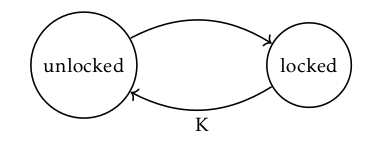
\includegraphics[width=200pt]{img/concurrency/transition-lock}
  \end{figure}
\end{itemize}

\subsubsection{Proofs}
There are 5 proof obligations to ensure that the implementation, predicates and tokens 
\begin{enumerate}
	\item $\text{isLock}(v,P,\gamma)$ is persistent since invariants and equality are persistent and conjunction and existential quantification preserves persistency
  \item $\text{locked}(\gamma)$ is not duplicable since $\Key \cdot \Key = \bot$ and therefore $\dboxed{\Key}^\gamma * \dboxed{\Key}^\gamma \vdash \dboxed{\Key \cdot \Key} ^ \gamma$ by \texttt{OWN-OP} which yields false by \texttt{OWN-VALID} by transitivity of $\vdash$ we are done 
  \item The specification of allocating a new lock is shown by showing the following triple
  \[
    \{P\} \text{newLock}() \{v.\exists \gamma . \text{isLock}(v,P, \gamma)\}
  \]
  by \texttt{HT-BETA} 
  \[
    \{P\} \iref(\false) \{v.\exists \gamma . \text{isLock}(v,P, \gamma)\}
  \]
  a new ghost state is allocated using \texttt{GHOST-ALLOC} and then \texttt{HT-CSQ} together with \texttt{HT-EXIST} and thus we are left with proving
  \[
    \{\text{locked}(\gamma) * P\} \iref(\false) \{v. \exists \gamma. \text{isLock}(v,P,\gamma)\}
  \]
  for some $\gamma$. Then the definition of locked is used
  \begin{equation*}
    \{\dbox{K}^\gamma * P\} \text{ref}(\text{false}) \{v. \exists \gamma. \text{isLock} (v, P, \gamma)\}
  \end{equation*}
  The \texttt{HT-BIND-DET} rule is used with an empty evaluation context. The following 
  \[
    \{\dbox{K} * P\} \text{ref}(\text{false}) \{v.\exists \ell. v= \ell \land \ell \hookrightarrow \text{false} * \dbox{K} * P\}
  \]
  is first proven as follows
  \[
  \begin{prooftree} 
    \infer0[\texttt{HT-ALLOC}]{\{\text{True}\} \text{ref}(\text{false}) \{v.\exists \ell. v= \ell \land \ell \hookrightarrow \text{false}\}}
    \infer1[\texttt{HT-FRAME}]{\{\dbox{K} * P\} \text{ref}(\text{false}) \{v.\exists \ell. v= \ell \land \ell \hookrightarrow \text{false} * \dbox{K} * P\}}
  \end{prooftree}
  \]
  Thus we are left with proving 
  \[
    \{\ell \hookrightarrow \text{false} * \dbox{K} * P\} \ell \{v. \exists \gamma. \text{isLock} (v, P, \gamma)\}
  \]
  where $\exists$I is used to get a concrete $\ell$ and it is proven as follows
  \[
  \begin{prooftree} 
    \infer0[\texttt{HT-RET}]{\{\text{True}\}  \ell \{v.v=\ell \}}
    \infer1[]{{\later(I(\ell, P, \gamma))\}  \ell \{v.\exists \iota . v=\ell \land \boxed{I(\ell, P, \gamma)}^\iota\}}}
    \infer1[\texttt{HT-CSQ}(1)]{{\later(I(\ell, P, \gamma))\}  \ell \{v.\exists \ell, \iota . v=\ell \land \boxed{I(\ell, P, \gamma)}^\iota\}}}
    \infer1[def.]{\{\later(\ell \hookrightarrow \text{false} * \dbox{K} * P \lor \ell\hookrightarrow \text{true})\}  \ell \{v.\exists \ell, \iota . v=\ell \land \boxed{I(\ell, P, \gamma)}^\iota\}}
    \infer1[\texttt{HT-CSQ}(2)]{\{\ell \hookrightarrow \text{false} * \dbox{K} * P\}  \ell \{v.\exists \ell, \iota . v=\ell \land \boxed{I(\ell, P, \gamma)}^\iota\}}
    \infer1[def.]{\{\ell \hookrightarrow \text{false} * \dbox{K} * P\} \ell \{v. \exists \gamma. \text{isLock} (v, P, \gamma)\}}
  \end{prooftree} 
  \]
  In \texttt{HT-CSQ}(1) $\exists$I and $\forall$I can be used to prove that the $\exists$ can be removed in the post condition. For \texttt{HT-CSQ}(2) should be proven 
  \[
    \vdash \ell \hookrightarrow \text{false} * \dbox{K} * P  \Rightarrow \later(\ell \hookrightarrow \text{false} * \dbox{K} * P \lor \ell\hookrightarrow \text{true})
  \]
  which can be proven as follows
  \[
  \begin{prooftree} 
    \infer0[\texttt{Asm.}]{\ell \hookrightarrow \text{false} * \dbox{K} * P  \vdash \ell \hookrightarrow \text{false} * \dbox{K} * P }
    \infer1[$\lor$IL]{\ell \hookrightarrow \text{false} * \dbox{K} * P  \vdash \ell \hookrightarrow \text{false} * \dbox{K} * P \lor \ell\hookrightarrow \text{true}}
    \infer1[$\later$weak]{\ell \hookrightarrow \text{false} * \dbox{K} * P  \vdash \later(\ell \hookrightarrow \text{false} * \dbox{K} * P \lor \ell\hookrightarrow \text{true})}
    \infer1[$\Rightarrow$I]{\vdash \ell \hookrightarrow \text{false} * \dbox{K} * P  \Rightarrow \later(\ell \hookrightarrow \text{false} * \dbox{K} * P \lor \ell\hookrightarrow \text{true})}
  \end{prooftree}
  \]
  \item The specification of the acquire operation is shown by first using the derived rule for recursive functions (from Exercise 6.4) i.e. assuming 
  \[
    \forall v, P, \gamma . \{\later \text{isLock}(v, P, \gamma)\} \text{acquire} \; v \{v.P * \text{locked}(\gamma)\}
  \]
  the following triple 
  \[
    \{\text{isLock}(v,P, \gamma) \} \iif \; \icas (v,\false,\true) \; \ithen \; () \; \ielse \; \text{acquire}(v) \{v.P * \text{locked}(\gamma)\}
  \]
  is shown. Using the $\text{isLock}(v,P,\gamma)$ together with \texttt{HT-PRE-EQ} and moving the invariant into the context we get the following
  \[
    \inv{I(\ell,P,\gamma)^\iota} \vdash \{\True\} \iif \; \icas (v,\false,\true) \; \ithen \; () \; \ielse \; \text{acquire}(\ell) \{v.P * \text{locked}(\gamma)\}
  \]
  then the cas expression is evaluated with the \texttt{HT-BIND} rule by first shown the following triple
  \[
    \inv{I(\ell,P,\gamma)^\iota} \vdash \{\True\} \icas (v,\false,\true) \{v.(u = \true * P * \text{locked}(\gamma) \lor (u = \false))\}
  \]
  since cas is atomic the \texttt{HT-INV-OPEN} rule can be used and thus it suffices to show that
  \begin{align*}
    &\{\later I(\ell, P, \gamma)\} \\
    \inv{I(\ell, P, \gamma)}^\iota \vdash \; & \quad \icas(\ell, \false, \true) \\
    &\{v.(u = \true * P * \text{locked}(\gamma) \lor (u = \false)) * I(\ell, P, \gamma)\}
  \end{align*}
  Then we case on the invariant using the \texttt{HT-DISJ} rule. For the first case
  \begin{align*}
    &\{\later (\ell \hookrightarrow \false * \text{locked} \; \gamma * P)\} \\
    \inv{I(\ell, P, \gamma)}^\iota \vdash \; & \quad \icas(\ell, \false, \true) \\
    &\{v.(u = \true * P * \text{locked}(\gamma) \lor (u = \false)) * I(\ell, P, \gamma)\}
  \end{align*}
  by \texttt{HT-CSQ} it suffices to establish either choice of the disjunctions in the postcondition. The following is chosen
  \[
    u = \true * P * \text{locked}(\gamma) * \ell \hookrightarrow \true 
  \]
  Which follows from using \texttt{HT-FRAME} and \texttt{HT-CAS-SUCC}. \smallskip \\
  In the second case we show
  \begin{align*}
    &\{\later (\ell \hookrightarrow \true)\} \\
    \inv{I(\ell, P, \gamma)}^\iota \vdash \; & \quad \icas(\ell, \false, \true) \\
    &\{v.(u = \true * P * \text{locked}(\gamma) \lor (u = \false)) * I(\ell, P, \gamma)\}
  \end{align*}
  which can be shown by \texttt{HT-CSQ} and establishing the following postcondition
  \[
    u = \false * \ell \hookrightarrow \true 
  \]
  and this follows from the \texttt{HT-CAS-FAIL} rule. \smallskip \\
  Then by the \texttt{HT-BIND} rule the following obligation remains
  \[
    \inv{I(\ell,P,\gamma)}^\iota \vdash \{u = \true * P * \text{locked}(\gamma) \lor u = \false\} \iif \; u \; \ithen \; () \; \ielse \; \text{acquire} \; \ell \{\_.P*\text{locked}(\gamma)\}
  \]
  The two cases in the precondition are considered using the \texttt{HT-DISJ} rule. Then the rules \texttt{HT-IF-TRUE} and \texttt{HT-IF-FALSE} is used on both cases and thus the following two things remains
  \begin{align*}
    &\inv{I(\ell, P, \gamma)^\iota} \vdash \{P * \text{locked}(\gamma)\} () \{\_. P * \text{locked}(\gamma)\} \\
    &\inv{I(\ell, P, \gamma)^\iota} \vdash \{\True\} \text{acquire} \; \ell \{\_. P * \text{locked}(\gamma)\} \\
  \end{align*}
  The first follows by the rule for the unit expressions and the second by the induction hypothesis. 
  \item The specification of the release operation by showing the following triple
  \[
    \{\text{isLock}(v,P, \gamma) * P * \text{locked}(\gamma)\} \text{release} \; v \{\_. \True\}
  \]
  Using the definition of $\text{isLock}(v,P,\gamma)$ the location governed by an invariant can be substituted into the expression under evaluation using the \texttt{HT-PRE-EQ} rule, and by the \texttt{HT-BETA} rule we get the following
  \[
    \{\inv{I(\ell, P, \gamma)}^\iota * \text{locked}(\gamma)\} \ell \leftarrow \false \{\_. \True\}
  \]
  Then the \texttt{HT-INV-OPEN} rule is used by moving the invariant into the assumption (since they are persistent) and thus we get the following triple
  \[
    \inv{I(\ell, P, \gamma)}^\iota \vdash \{\later I(\ell, P, \gamma) * P * \text{locked}(\gamma)\} \ell \leftarrow \false \{\_. \later I(\ell, P, \gamma)\}
  \]
  The two cases in the disjunction in $I(\ell, P, \gamma)$ are considered in the precondition. The first case is 
  \[
    \inv{I(\ell, P, \gamma)}^\iota \vdash \{\later (\ell \hookrightarrow \false * \text{locked}(\gamma) * P) * P * \text{locked}(\gamma)\} \ell \leftarrow \false \{\_. \later I(\ell, P, \gamma)\}
  \]
  which is inconsistent as $\text{locked} * \text{locker} \vdash \False$ and thus it follows by \texttt{HT-LATER-FALSE} \smallskip \\
  For the second case
  \[
    \inv{I(\ell, P, \gamma)}^\iota \vdash \{\later (\ell \pointsto \true) * P * \text{locked}(\gamma)\} \ell \leftarrow \false \{\_. \later I(\ell, P, \gamma)\}
  \]
  and in the postcondition the first disjunct is chosen by \texttt{HT-CSQ} and in the precondition the $\later$\texttt{-LATER} is used to get $\later$ 
  \[
    \inv{I(\ell, P, \gamma)}^\iota \vdash \{\later (\ell \pointsto \true) * \later (P * \text{locked}(\gamma))\} \ell \leftarrow \false \{\_. \later (\ell \pointsto \false) * \later(\text{locked}(\gamma) * P)\}
  \]
  which holds by the \texttt{HT-FRAME} and \texttt{HT-STORE}
\end{enumerate}

% \subsection{Bags}
% TODO?

\newpage
%%% Local Variables:
%%% mode: latex
%%% TeX-master: "pav-noter"
%%% End:

\section{Concurrency: Counter Modules}
\subsection{Later and persistent modalities}
\begin{itemize}
  \item The $\later$ modality expresses that a property is only supposed to hold later, after a reduction step has taken place
	\item The set of Iris proportions is not just a set of resources
  \begin{itemize}
  	\item An iris proposition $P$ is closer to being a set of pairs $(k,r)$ where $k$ is a natural number and $r$ a reource
    \item $k$ can be thought of as a step-index i.e. a natural number which expresses for how many reduction steps we know that $r$ is in $P$ 
    \item If $(k,r) \in P$ and $m \leq k$ then also $(m,r) \in P$ 
    \item The step-indices are used to interpret $\later$
    \[
      \later P=\{(m+1, r) \mid (m, r) \in P\} \cup\{(0, r) \mid r \in \mathcal{R}\}
    \]
    \item ``later'' means that the index number is smaller 
    \begin{itemize}
    	\item There are fewer reductions steps left after some reduction steps has been taken
    \end{itemize}
  \end{itemize}
  \item The persistent modality $\square$ is defined as follows
  \[
    \square P=\left\{r \in \mathcal{R} | \exists s, r^{\prime}, s \in P \wedge s=s \cdot s \wedge r=s \cdot r^{\prime}\right\}
  \]
  \begin{itemize}
  	\item $\square P$ is the upwards-closure of the set of duplicable resources in $P$
    \item Persistent predicates are those predicates that do not assert exclusive owner, over resources
    \item It only expresses ``knowledge'' and now exclusive ownership
    \item Persistent predicates $P$ are duplicable: $P \dashv\vdash P * P$
  \end{itemize}
  % TODO persistent rule for moving 
  \item There are two kinds of primitive persistent propositions 
  \[
    t =_\tau t' \dashv \vdash \square (t =_\tau t') \quad \{P\} e \{\Phi\} \dashv \vdash \square \{P\} e \{\Phi\}
  \]
  \item The rule \texttt{HT-PERSISTENTLY} can be used to move persistent propositions in and out of preconditions
  \[
  \begin{prooftree} 
    \hypo{\square Q \land S \vdash \{P\}\; e \; \{v.R\}}
    \infer[double]1{S \vdash \{P \land \square Q\}\; e \; \{v.R\}} 
  \end{prooftree}
  \]
\end{itemize}

\subsection{Proof rules}
\begin{itemize}
	\item $e_1 \mid \mid e_2$ runs $e_1$ and $e_2$ is parallel, waits until both finish, and then returns a pair consisting of the values to which $e_1$ and $e_2$ evaluated 
  \begin{itemize}
  	\item It is definable using fork
  \end{itemize}
  \item The following rule \texttt{HT-PAR}
  \[
  \begin{prooftree} 
    \hypo{S \vdash \{P_1\}e_1 \{v.Q_1\}}
    \hypo{S \vdash \{P_2\}e_2 \{v.Q_2\}} 
    \infer2{S \vdash \{P_1 * P_2\} e_1 \mid \mid e_2 \{v. \exists v_1v_2.v = (v_1,v_2) * Q_1[v_1/v] * Q_2[v_2/v]\}} 
  \end{prooftree}
  \]
  states that one can run $e_1$ and $e_2$ in parallel and if they have \textbf{disjoint} footprints and then verify the two components seperately 
  \begin{itemize}
    \item It is referred to as the \textbf{disjoint concurrency rule}
    \item Each thread is reasoned about in isolation (\textbf{thread-local reasoning}) 
  	\item Important since it is not possible to reason about all possible interleavings of threads since there are too many
  \end{itemize}
  % HT-CAS construct and rule 
  \item The following rule \texttt{HT-CAS}
  \[
  \begin{prooftree} 
    \infer0{\{\later \ell \hookrightarrow v\} \text{cas}(\ell,v_1,v_2)\{u.(u = \true * v = v_1 * \ell \hookrightarrow v_2) \lor (u = \false * v \neq v_1 * \ell \hookrightarrow v)\}} 
  \end{prooftree}
  \]
  is used for the general case of the cas primitive. 
  \begin{itemize}
    \item The derived rules \texttt{HT-CAS-SUCC}
    \[
    \begin{prooftree} 
      \infer0{\{\later \ell \hookrightarrow v_1\} \text{cas}(\ell,v_1,v_2)\{u.u = \true * v = v_1 * \ell \hookrightarrow v_2\}} 
    \end{prooftree}
    \]
    and \texttt{HT-CAS-FAIL} 
    \[
    \begin{prooftree} 
      \infer0{\{\later \ell \hookrightarrow v * \later(v \neq v_1)\} \text{cas}(\ell,v_1,v_2)\{u.u = \false * \ell \hookrightarrow v\}} 
    \end{prooftree}
    \]
    are often easier to use
  \end{itemize}
\end{itemize}
%%% Local Variables:
%%% mode: latex
%%% TeX-master: "pav-noter"
%%% End:

   
\subsection{Counter modules and authoritative resource algebra}
\begin{itemize}
	\item A situation is considered where several threads operate on shared state
  \item Each thread has a partial view of the shared state
  \item There is an invariant governing the shared state
  \item The invariant keeps track of what the actual state is (authoritative view)
\end{itemize}

\subsubsection{Requirements}
\begin{itemize}
  \item The counter module has three methods
  \begin{itemize}
  	\item newCounter for creating a fresh counter 
    \item incr for increasing the value of the counter
    \item read for reading the current value of the counter
  \end{itemize}
  \item There is an abstract predicate $\text{isCounter}(v,n)$ which states that $v$ is a couter whose value is $n$
  \begin{itemize}
  	\item It should be persistent such that it can be shared between threads 
    \item It canot state that $n$ is exactly the value of the counter but only its lower bound
  \end{itemize} 
\end{itemize}

\subsubsection{Implementation}
\begin{itemize}
	\item The newCounter method creates the counter which is a location containing the counter value
  \[
    \text{newCounter}() = \iref(0)
  \]
  \item The incr method increases the value of the counter by 1 (done by a cas loop since $\ell \leftarrow !\ell + 1$ is not an atomic operation)
  \begin{align*}  
    \irec \; \text{incr}(\ell) = &\ilet \; n=!\ell \; \iin \\
                                 &\ilet \; m = n+1 \; \iin \\
                                 &\iif \; \icas(\ell, n,m) \; \ithen \; () \; \ielse \; \text{incr} \; \ell
  \end{align*}
  \item The read method just reads the value
  \[
    \text{read} \; \ell = !\ell
  \]
\end{itemize}

\subsubsection{Resource algebra requirements}
\begin{itemize}
	\item An invariant is used to keep track of the shared state of the module i.e. the value of the counter
  \item The invariant will have the \textbf{authoritative view} of the value of the counter, a ghost assertion
  \[
    \dboxed{\auth m}^\gamma
  \]
  this is intuitively the true value of the counter
  \item Each thread will have a fragmental view of the counter value which is captured by the ghost assertion
  \[
    \dboxed{\prt n}^\gamma
  \]
  this is intuitively a lower bound of the correct, true, value of the counter
  \item The abstract predicate is defined as
  \[
    \text{isCounter}(\ell, n, \gamma) = \dboxed{\prt n}^\gamma * \exists \iota.\inv{\exists m. \ell \pointsto m * \dboxed{\auth m}^\gamma}^\iota
  \]
  which can be used to define the counter specification as follows
  \begin{align*}
    &\{\True\} \text{newCounter}() \{u.\exists \gamma.\text{isCounter}(u,0,\gamma)\} \\
    &\forall \gamma. \forall v. \forall n. \{\text{isCounter}(v,n,\gamma)\} \; \text{read} \; v \; \{u.u \geq n\} \\
    &\forall \gamma. \forall v. \forall n. \{\text{isCounter}(v,n,\gamma)\} \; \text{incr} \; v \; \{u.u = () * \text{isCounter}(v, n+1, \gamma)\}
  \end{align*}

  \item The requirements for the resource algebra is
  \begin{enumerate}
    \item A fragmental view should be duplicable i.e.
    \[
      | \prt n | = \prt n \\
    \]
    \item The fragmental view is the lower bound of the true value 
    \[
      \auth m \cdot \prt n \in \mathcal V \Rightarrow m \geq n
    \]  
    \item If one both owns the authoritative view and a fragmental view, then we may update them
    \[
      \auth m \cdot \prt n \leadsto \auth (m + 1) \cdot \prt (n + 1)
    \]
  \end{enumerate}
\end{itemize}

\subsubsection{Resource algebra definition}
\begin{itemize}
	\item Carrier: $\mathcal M = \mathbb N_{\bot, \top} \times \mathbb N$ where $\mathbb N_{\bot, \top}$ is the natural numbers with two additional element $\bot$ and $\top$ 
  \item For $m,n \in \mathbb N$, write $\auth m$ for $(m,0)$ and $\prt n$ for $(\bot, n)$
  \item Operation:
  \[
    (x,n) \cdot (y, m) = 
    \begin{cases} 
      (y, \max(n,m))    & \text{if } x = \bot \\ 
      (x, \max(n,m))    & \text{if } y = \bot \\ 
      (\top, \max(n,m)) & \text{otherwise}
    \end{cases}
  \]
  \item The unit is $(\bot, 0)$
  \item The valid set is defined as follows
  \[
    \mathcal V = \{(x,n) \mid x = \bot \lor x \in \N \land x \geq n\}
  \]
  \item The core is defined as
  \[
    |(x,n)| = (\bot, n)
  \]
  \item $(\mathcal M, \mathcal V, |\cdot |)$ is a unital resource algebra
  \item $\auth m \cdot \prt n \leadsto \auth (m+1) \cdot \prt (n+1)$
\end{itemize}

\subsubsection{A More General Authoritative Resource Algebra}
\begin{itemize}
  \item Given a unital resource algebra $(\mathcal M, \epsilon, \mathcal V, | \cdot |)$ let $\text{AUTH}(\mathcal M)$ be the following resource algebra
  \begin{itemize}
    \item Carrier $\mathcal M_{\bot, \top} \times \mathcal M$ 
    \item The operation 
    \[
      (x, a) \cdot (y, b) = 
      \begin{cases} 
        (y, a \cdot b) & \text{if } x = \bot \\
        (x, a \cdot b) & \text{if } y = \bot \\
        (\top, a \cdot b) & \text{otherwise}
      \end{cases}
    \]
    \item The core is defined as 
    \[
      \mathcal V_{\text{AUTH}(\mathcal M)} \left\{(x, a) \mid x = \bot \land a \in \mathcal V \lor x \in \mathcal M \land x \in \mathcal V \land a \preccurlyeq x \right\}
    \]
  \end{itemize}
  \item Properties of $\text{AUTH}(\mathcal M)$
  \begin{itemize}
    \item \texttt{AUTH}$(\mathcal M)$ is unital with unit $(\bot, \epsilon)$ where $\epsilon$ is the unit of $\mathcal M$ \smallskip \\
    \textbf{Proof} it is first seen that \texttt{AUTH}$(\mathcal M)$ is commutative. This follows from the way the operation is specified. The operation on the first element is clearly commutative since it is just the identity function on the element which is not $\bot$ if this element does exists. The second part of the element relies on the $\mathcal M$ being commutative which it is. \bigskip \\
Then it is seen that the unit is $(\bot, \epsilon)$ since for another element $(x,y)$ from the carrier the following holds
    \begin{equation*}
      (\bot, \epsilon) \cdot (x,y) = (x, \epsilon \cdot y) = (x,y)
    \end{equation*}
    Then since \texttt{AUTH}($\mathcal M$) is commutative it must also hold that $(\bot, \epsilon) \cdot (x,y) = (x,y)$ and therefore it must be the unit element. It is clear that $(\bot, \epsilon) \in \mathcal \mathcal V_{\mathtt{AUTH}(\mathcal M)}$ since the first part is $\bot$. The property $|(\bot, \epsilon)| = (\bot, \epsilon)$ holds since
   \begin{equation*}
     |(\bot, \epsilon)| = (\bot, |\epsilon|) = (\bot, \epsilon)
   \end{equation*}
  Thereby \texttt{AUTH}$(\mathcal M)$ must be unital, since all properties hold.
  \item $\bullet x \cdot \bullet y \notin \mathcal V_{\mathtt{AUTH}(\mathcal M)}$ \smallskip \\
  \textbf{Proof} It follows since the first part of both elements is not $\bot$ therefore the resulting element of the operation is one the form $(\top, y)$ which is not valid. Since the first part should either be an element in $\mathcal M$ or the element $\bot$ for the whole element to be valid.
  \item $\cdot \circ x \cdot \circ y=\circ(x \cdot y)$ \smallskip \\
  \textbf{Proof}
  \begin{align*}
    \circ x \cdot \circ y = (\bot, x) \cdot (\bot, y) = (\bot, x \cdot y) = \circ(x \cdot y)
  \end{align*}
  \item $\bullet x \cdot \circ y \in \mathcal{V} \Rightarrow y \preccurlyeq x$ \smallskip \\
  \textbf{Proof}
  \begin{align*}
     \bullet x \cdot \circ y \in \mathcal{V} &\Rightarrow (x,y) \in \mathcal V \text{ for } x \neq \bot \\
                                             &\Rightarrow (x,y) \in \{(x,a) \mid x = \bot \land a \in \mathcal V \lor x \in \mathcal M \land x \in \mathcal V \land a \curlyeqprec x\} \text{ for } x \neq \bot \\
                                             &\Rightarrow x = \bot \land a \in \mathcal V \lor x \in \mathcal M \land x \in \mathcal V \land a \curlyeqprec x \text{ for } x \neq \bot \\
                                             &\Rightarrow  x \in \mathcal M \land x \in \mathcal V \land a \curlyeqprec x \Rightarrow a \curlyeqprec x \
  \end{align*}
  \item If $x \cdot z$ is valid in $\mathcal M$ then
  \[
    \bullet x \cdot \circ y \leadsto \bullet(x \cdot z) \cdot \circ(y \cdot z)
  \]
  in \texttt{AUTH}$(\mathcal M)$ \smallskip \\
  \textbf{Proof} It follows from part 4 since if $\bullet x \cdot \circ y$ is valid if and only if $\bullet(x \cdot z) \cdot \circ(y \cdot z) = (x \cdot z, y \cdot z)$ since they are only invalid if it is not the case that $y \preccurlyeq x$. Since the differences between the two elements are the same it is impossible to find a element $(a,b)$ where $y \cdot b \preccurlyeq x \cdot a$ and where $y \cdot z \cdot b \preccurlyeq x \cdot z \cdot a$ does not hold.
  \item If $x \cdot z$ is valid in $\mathcal{M}$ and $w \preccurlyeq z$ then
  \[
    \bullet x \cdot \circ y \leadsto \bullet(x \cdot z) \cdot \circ(y \cdot w)
  \]
  in \texttt{AUTH}$(\mathcal M)$ \smallskip \\
  \textbf{Proof} It follows from part 4 since if $\bullet x \cdot \circ y$ is valid if and only if $\bullet(x \cdot z) \cdot \circ(y \cdot z) = (x \cdot z, y \cdot w)$ since they are only invalid if it is not the case that $y \preccurlyeq x$. Since the difference between the first elements are bigger than for the second element it is impossible to find a element $(a,b)$ where $y \cdot b \preccurlyeq x \cdot a$ and where $y \cdot z \cdot b \preccurlyeq x \cdot z \cdot a$ does not hold.
  \end{itemize}
\end{itemize}

\subsubsection{A More Precise Specification}
\begin{itemize}
	\item To get a more precise specification a fraction $q$ is added to the abstract isCounter predicate
  \begin{itemize}
  	\item The intuition is that if a thread has owner ship of $\text{isCounter}(\ell, n \gamma, q)$ then the contribution of this thread to the actual counter value is $n$ and if $q=1$ then the thread is the sole owner, otherwise $(q < 1)$ then one have fragmental ownership
  \end{itemize}
  \item Using this one can get the following specification more precise definition
  \begin{align*}
    &\{\True\} \; \text{newCounter}() \{u. \exists \gamma. \text{isCounter}(u,0,\gamma,1)\} \\
    &\forall p. \forall \gamma. \forall v. \forall n. \{\text{isCounter}(v,n,\gamma, p)\} \; \text{read} \; v \; \{u.u \geq n\} \\
    &\forall \gamma. \forall v. \forall n. \{\text{isCounter}(v,n,\gamma, p)\} \; \text{read} \; v \; \{u.u = n\} \\
    &\forall p. \forall \gamma. \forall v. \forall n. \{\text{isCounter}(v,n,\gamma, p)\} \; \text{incr} \; v \; \{u.u = () * \text{isCounter}(v,n+1,\gamma,p)\}
  \end{align*}
  \item isCounter is not instead we have the following
  \[
    \text{isCounter}(\ell, n+k, \gamma, p + q) \dashv \vdash \text{isCounter}(\ell, n, \gamma, p) * \text{isCounter}(\ell, k, \gamma, q)
  \]
\end{itemize}

\newpage
%%% Local Variables:
%%% mode: latex
%%% TeX-master: "pav-noter"
%%% End:


\end{document}
%%% Local Variables:
%%% mode: latex
%%% TeX-master: t
%%% End:
